%!TEX root = ../thesis.tex

\chapter{Results}
\label{ch:results}

\section{Production profile}


\subsection{Tilt angle and azimuth}
The loss factors that show to be greatest is the mounting of the panel. Some panels where re-mounted during the interviews, as they were tilted the wrong way for optimal production. Although a lot of them were helped in the placing of the system, the tilt and azimuth varied for each system. Figure \ref{result:fig:slope_efficiency} shows that there is no correlation between the slope efficiency\footnote{The slope efficiency is calculated using a yearly total sum of energy produced with different slopes from \citep{huldNewSolarRadiation2012}} of the panels, and if they were helped or not. The average efficiency loss from the system was 21\%. 

\begin{minipage}[t]{0.5\textwidth} % Adjust width as needed
    \begin{figure}[H]
        \centering
        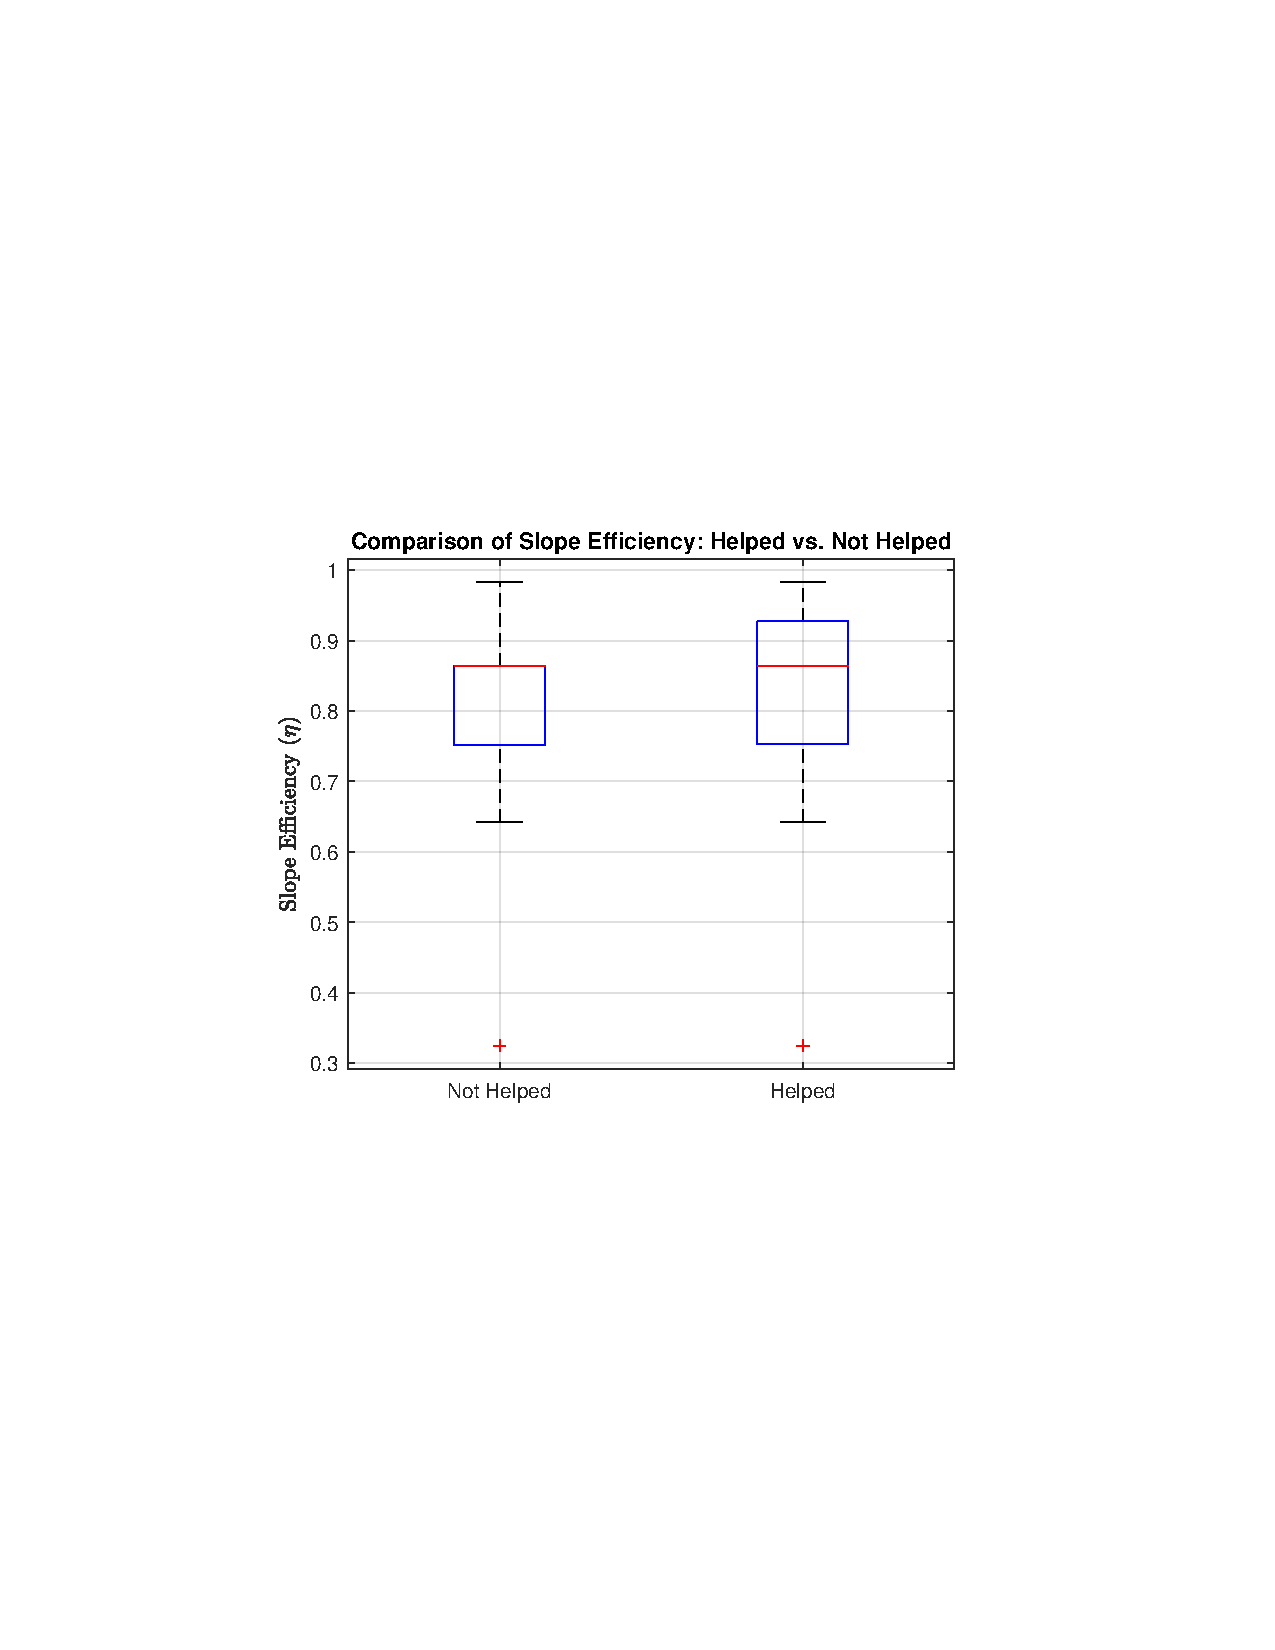
\includegraphics[width=\linewidth]{photos/SlopeEfficiency.pdf} %% Gjer denna om til kryss og sirkel
        \caption{Slope efficiency in a box plot. Red line is the median, the blue box contains the middle 50\% of data points and the red crosses are outliers.}
        \label{result:fig:slope_efficiency}
    \end{figure}
\end{minipage}% <--- IMPORTANT: The '%' symbol prevents unwanted horizontal space
%\hspace{0.01\textwidth}% Adjust this to control the horizontal space between figure and table
\begin{minipage}[t]{0.5\textwidth} % Adjust width so (width1 + hspace + width2) is about 1.0\textwidth
\vspace{0.05\textwidth}
    \begin{table}[H]
        \centering
        \small % To match the font size of your example table
        % Define the new table based on the updated image data
        % The \linewidth here refers to the width of this minipage (0.46\textwidth)
        \begin{tabularx}{\linewidth}{|>{\RaggedRight\arraybackslash\hsize=0.40\hsize}X|>{\Centering\arraybackslash\hsize=0.20\hsize}X|>{\Centering\arraybackslash\hsize=0.20\hsize}X|>{\Centering\arraybackslash\hsize=0.20\hsize}X|}
        \hline
        % Title row for the table (not bold, matching your example's multicolumn style)
        \multicolumn{4}{|c|}{Placement Effectiveness Data} \\
        \hline
        % Column Headers with math mode as requested
        Placement & \textbf{$\phi$} & \textbf{$\alpha$} & \textbf{$\eta$} \\
        \hline
        % Data rows from the new image, in the specified order
        % Assuming "Angled $$S" is "Angled $S$" and "Vertial" is "Vertical"
        % Interpreting "Angled" and "$S_E$" on subsequent lines as "Angled $S_E$"
        Angled $S$ & 0 & 35 & 0.98 \\ \hline
        Angled $S$ & 0 & 45 & 0.97 \\ \hline
        Angled $S_E$ & -45 & 20 & 0.89 \\ \hline
        Horizontal & 0 & 0 & 0.86 \\ \hline
        Angled $S_E$ & -45 & 35 & 0.86 \\ \hline
        Vertical $S$ & 0 & 90 & 0.64 \\ \hline
        Vertical $E$ & -90 & 90 & 0.33 \\ \hline
        \end{tabularx}
        \caption{Effectiveness of different azimuth ($\phi$) and slope ($\alpha$) combinations. ($\eta$) is efficiency where $\eta=1$ is the optima}
        \label{table:placement_effectiveness_data_new} % Choose a new unique label
    \end{table}
\end{minipage}

This could be due to the lack of experience of angle and azimuth from the installers, and perhaps a fear from the participants of changing the setup of the donated system.  

\subsection{Cleaning}
When asked if they had cleaned the panel, only one system was cleaned out of 19 in the study. Most explained that they did not want to touch the panels, as they were afraid to break them. Most panels did not look visibly soiled, and were often placed on roofs away from the dust. The region is not an arid region, and as mentioned in chapter \ref{ch:theory}, it will not be subject to heavy soiling. Although not in a heavy soiling environment, they will still be soiled and need washing to have full effect. As found in chapter \ref{ch:theory}, the soiling in mild regions will cause about a 10\% reduction in efficiency. 

\subsection{Simulation results}
In figure \ref{result:fig:Production_Simulation_results_summer&winter} we see the average production with all loss factors included. The graph shows the difference between the panels for the systems, with their effectiveness range from installation as well. Both duration and peak is significantly lower in the winter season than the summer season, justifying the need for two scenarios. The wide shaded region shows how much the installation process matters for the production of the panel. In general the effectiveness is still high, even though the average has not accounted for low $\eta$ outliers. 
\begin{figure}[H]
    \centering
    \begin{minipage}[t]{0.48\textwidth} % Adjust width as needed
        \centering
        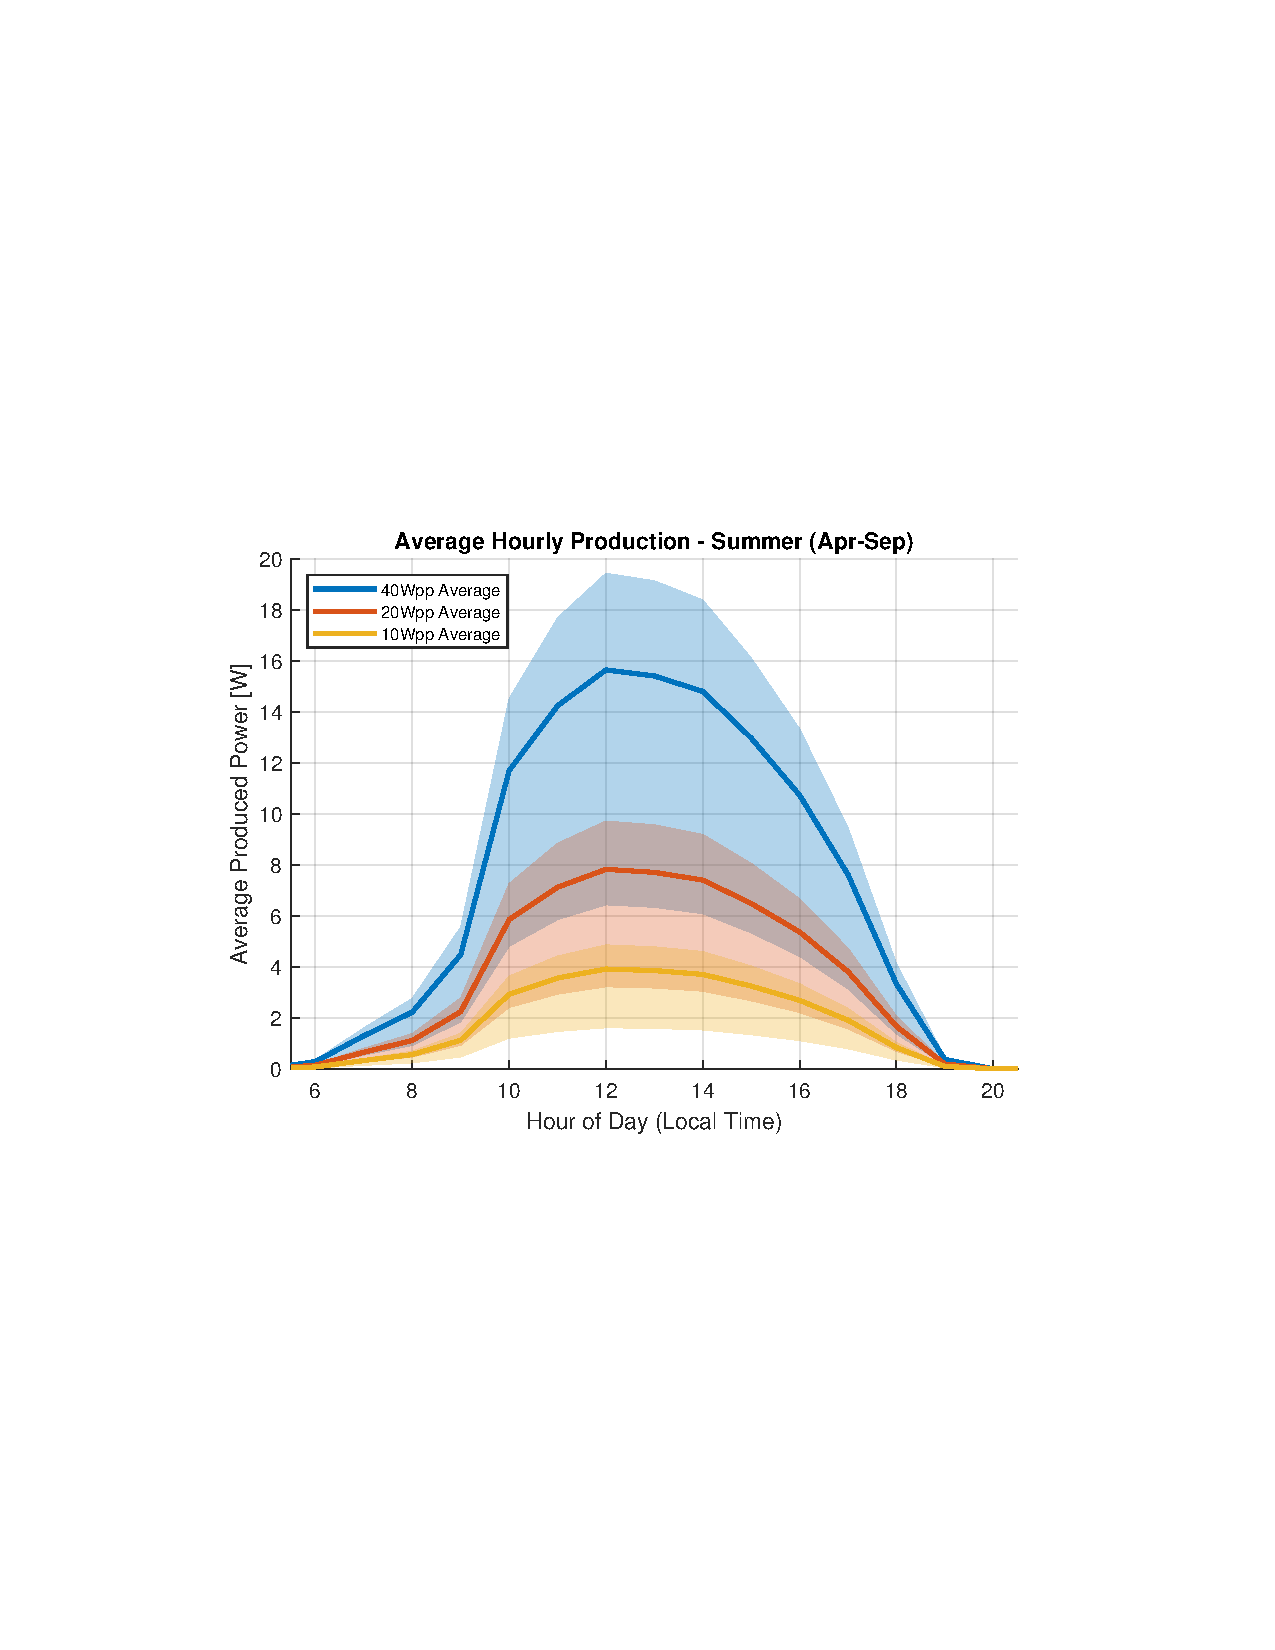
\includegraphics[width=\linewidth]{photos/Average_production_with_eta&soiling&loss_shaded_allPanels_Summer.pdf} %% Gjer denna om til kryss og sirkel
    \end{minipage}%
    \hspace{0.02\textwidth}% Adjust this to control the horizontal space between figure and table
    \begin{minipage}[t]{0.48\textwidth} % Adjust width so (width1 + hspace + width2) is about 1.0\textwidth
        \centering
        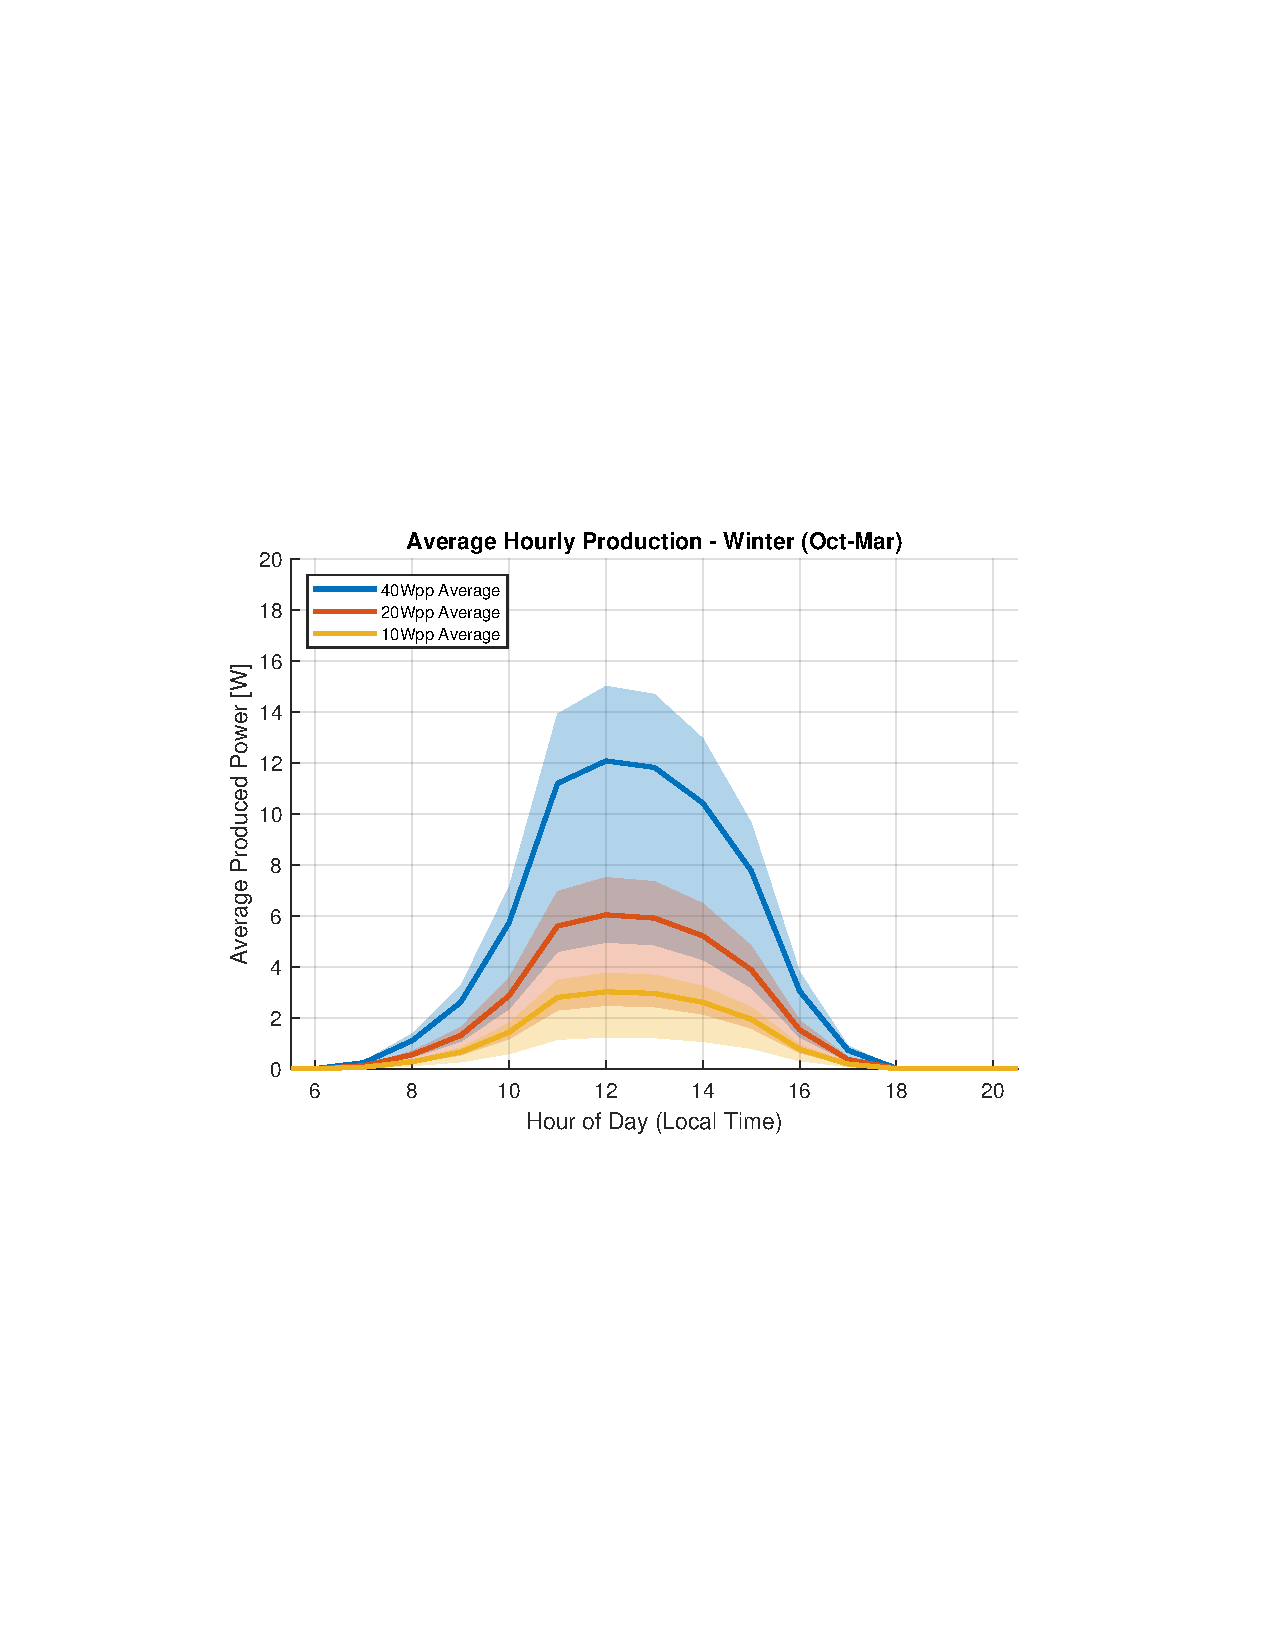
\includegraphics[width=\linewidth]{photos/Average_production_with_eta&soiling&loss_shaded_allPanels_Winter.pdf} %% Gjer denna om til kryss og sirkel
    \end{minipage}
    \caption{Summer and winter average production with loss factors. Soiling 10\%, general transmission loss 14\%. Shaded area represents the area between the most and least effective $\eta$ based on installation, data from table \ref{table:placement_effectiveness_data_new}. The line is the average of the data vectors in the area.}
    \label{result:fig:Production_Simulation_results_summer&winter}
\end{figure}


\section{Daily load profile}
The consumption data for the daily load profile is not as precise as it could be, if there was data logging on the systems. Some of the data needed to be estimated from the interview data and some weather data for sunrise and sunset. We end up with having two different dataset, one for winter and one for summer. These two sets show what we also see from the graph of national consumption on figure \ref{method:fig:gridloadalbania}, that winter months have higher load than summer months. 
\subsection{Consumption profile}
Figure \ref{result:fig:mean_power_allsystems_with95CI} shows the average power drain during 24-hours, derived from the consumption data of all systems. The consumption seems to follow the duck curve referenced in \ref{ch:method}. Having a lower consumption during the midday, when the power generation is highest. Different from the duck curve and the national grid load, the SHS has more load during the night. As the SHS supplies mainly light, this corresponds to the intended usage. 

\begin{figure}[H] % Using [H] as per your code; consider [!htbp] for production
    \centering % Center the entire figure block on the page

    % Left Column: Main Figure
    \begin{subfigure}[t]{0.52\linewidth} 
        \vspace*{0pt} % Ensures the reference point for [t] alignment is the very top
        \centering
        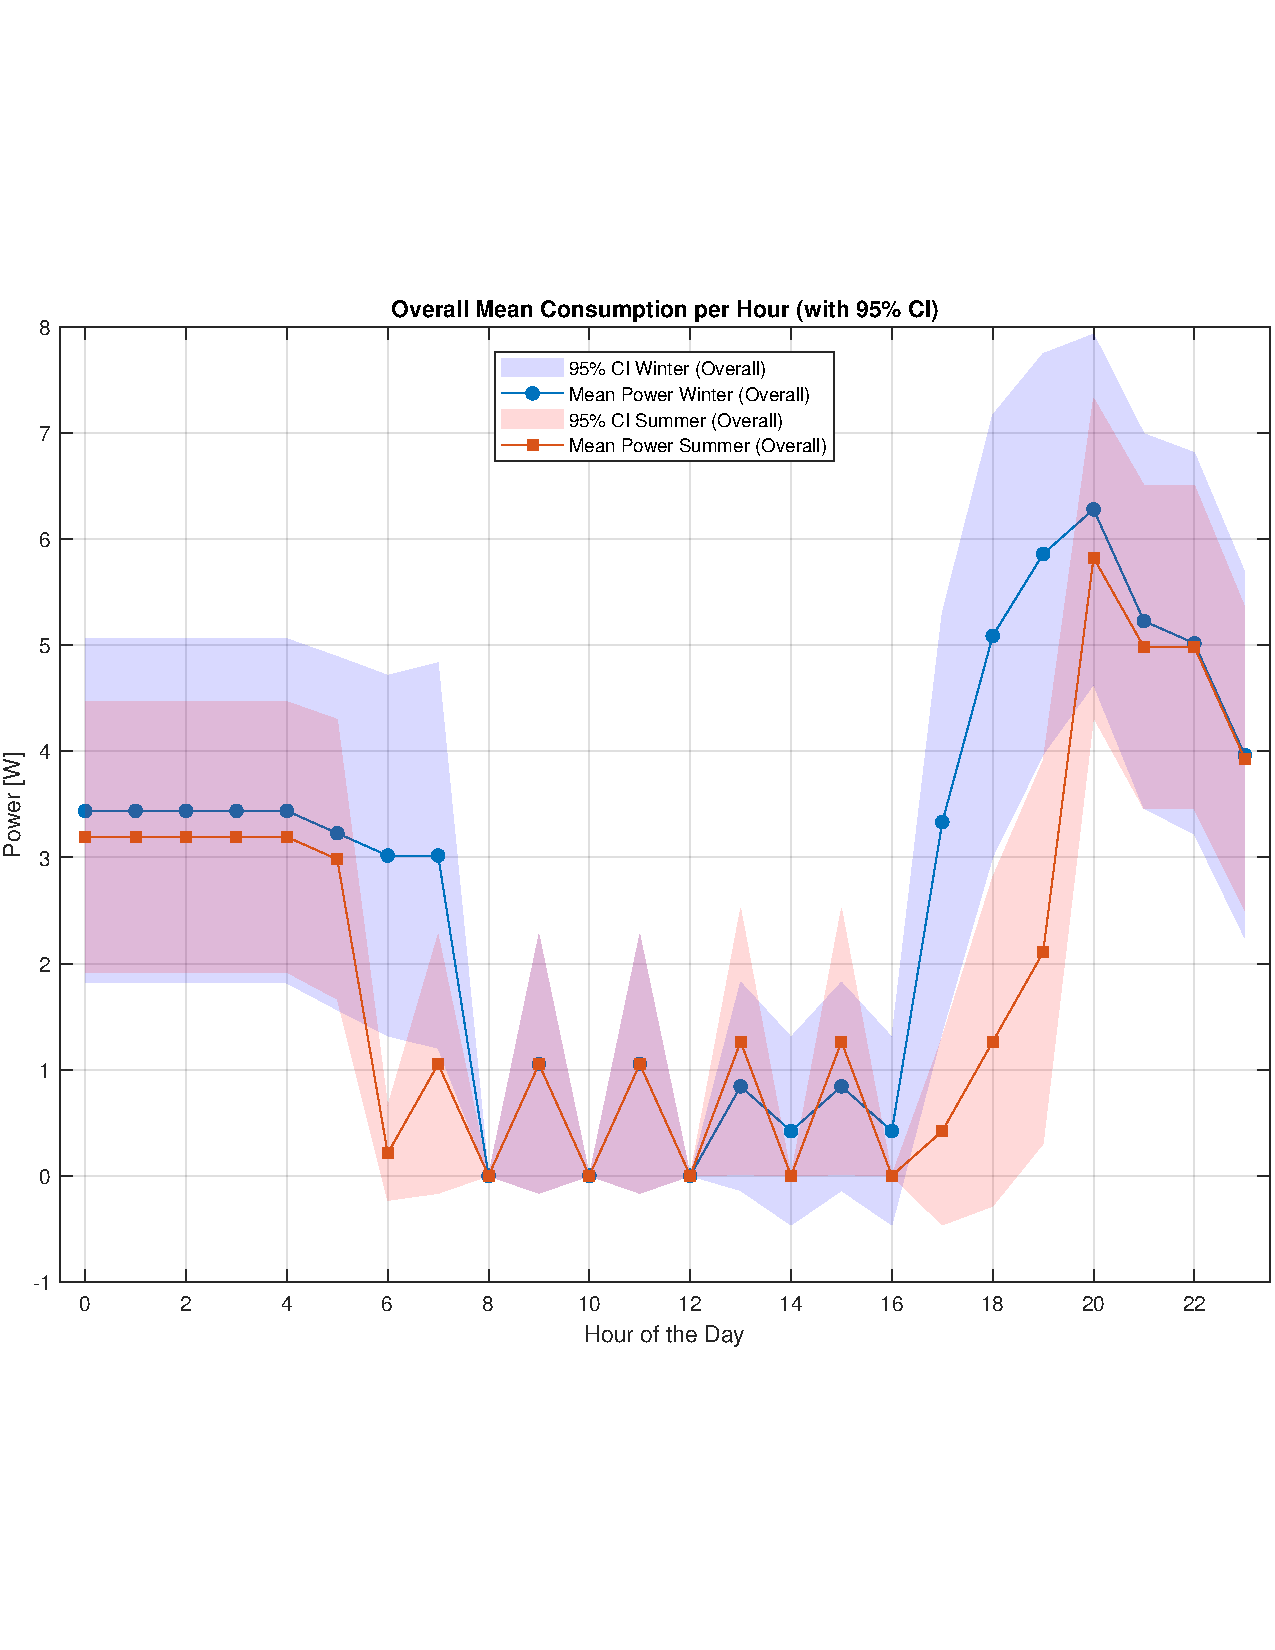
\includegraphics[width=\linewidth, height=\LeftImageHeight, keepaspectratio]{photos/Mean_consumption_winter&summer_all_systems_with_95CI.pdf}
        %\captionsetup{font=footnotesize}
        %\caption{Mean consumption from all systems during summer and winter. 95\% confidence interval applied.}
        %\label{result:fig:mean_power_allsystems_with95CI}
    \end{subfigure}\hfill % \hfill creates a flexible horizontal space
    % Right Column: Stack of Three Figures
    \begin{minipage}[t]{0.45\linewidth} 
        \vspace*{0pt} % Ensures the reference point for [t] alignment is the very top
        \centering 
        \begin{subfigure}{\linewidth} 
            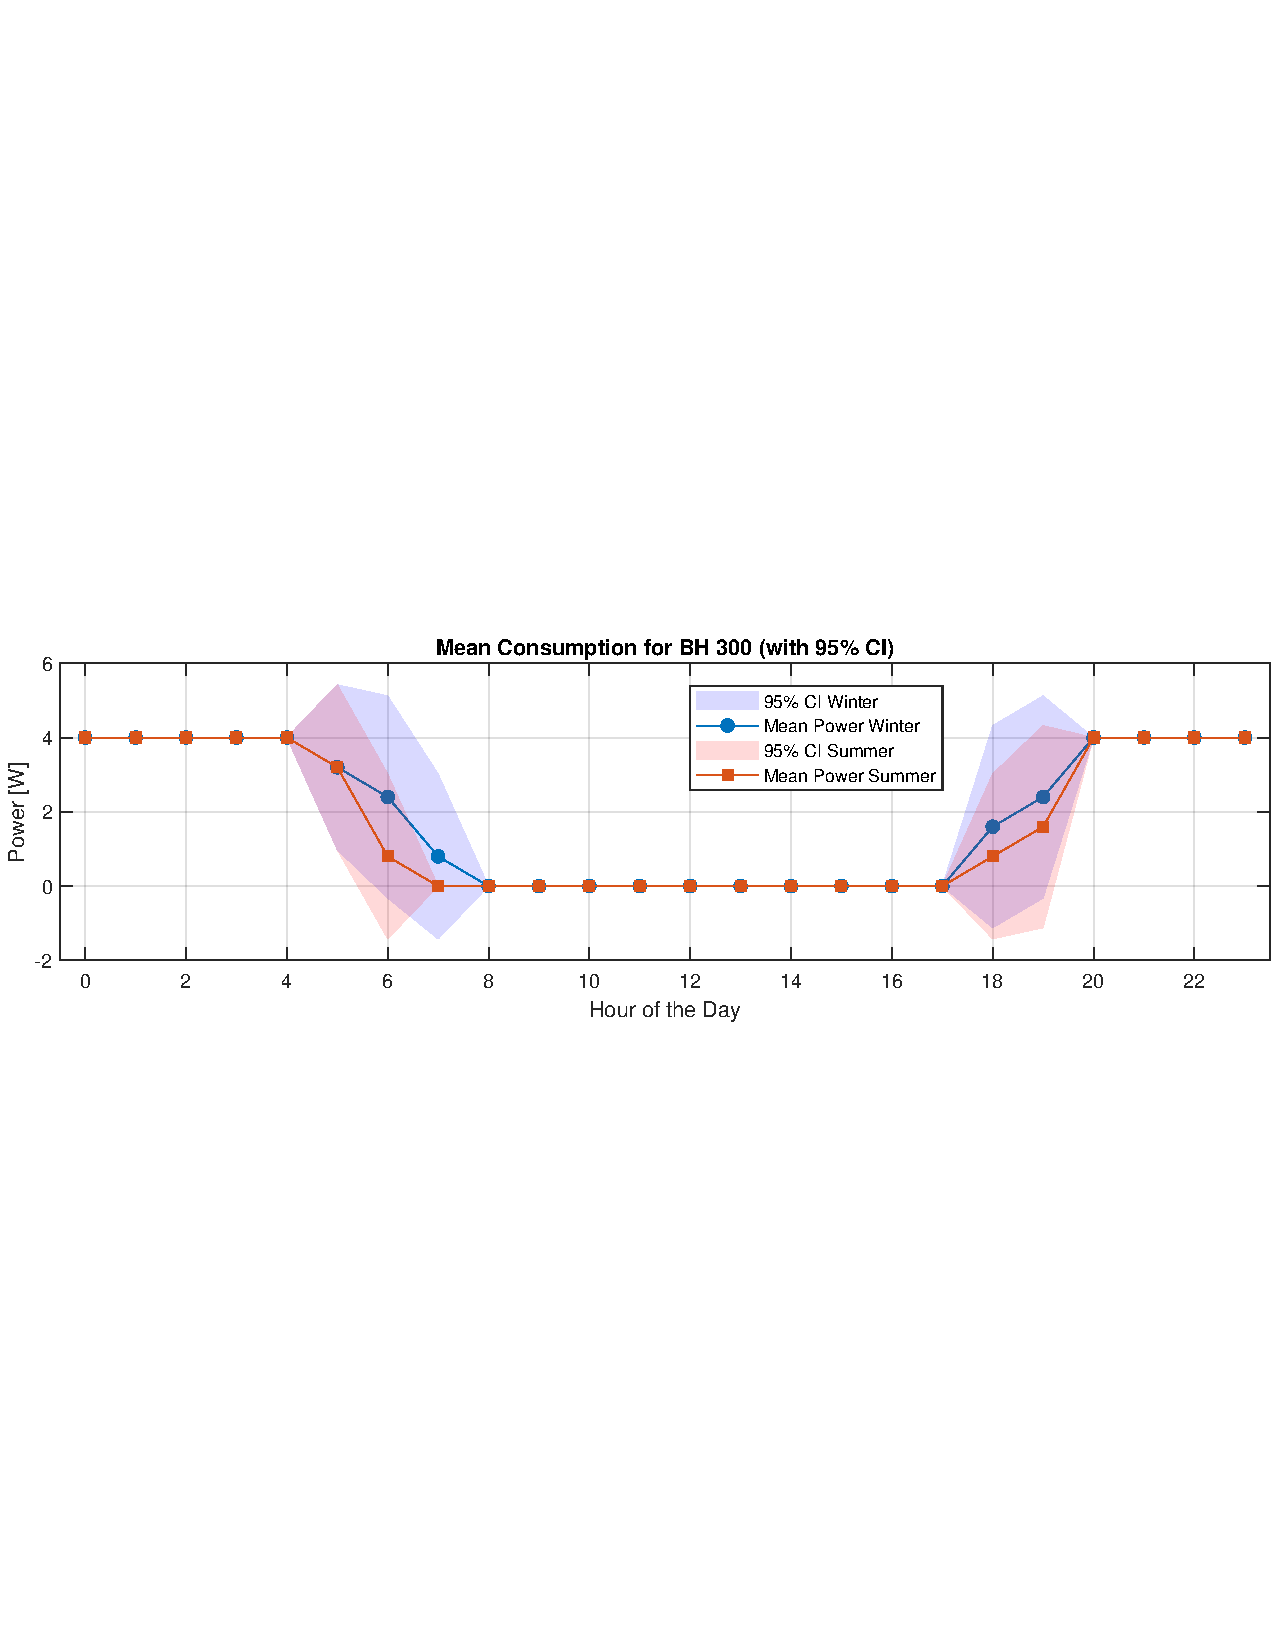
\includegraphics[width=\linewidth, height=\RightImageEachHeight, keepaspectratio]{photos/Mean_consumption_winter&summer_system1_with_95CI.pdf}
            %\captionsetup{font=tiny}
            %\caption{Consumption for System 1 with CI (Example)}
            %\label{fig:system1_CI}
        \end{subfigure}
        \par\vspace{\RightImageVSpace} % \par ensures \vspace is inter-paragraph space if needed
        \begin{subfigure}{\linewidth}
            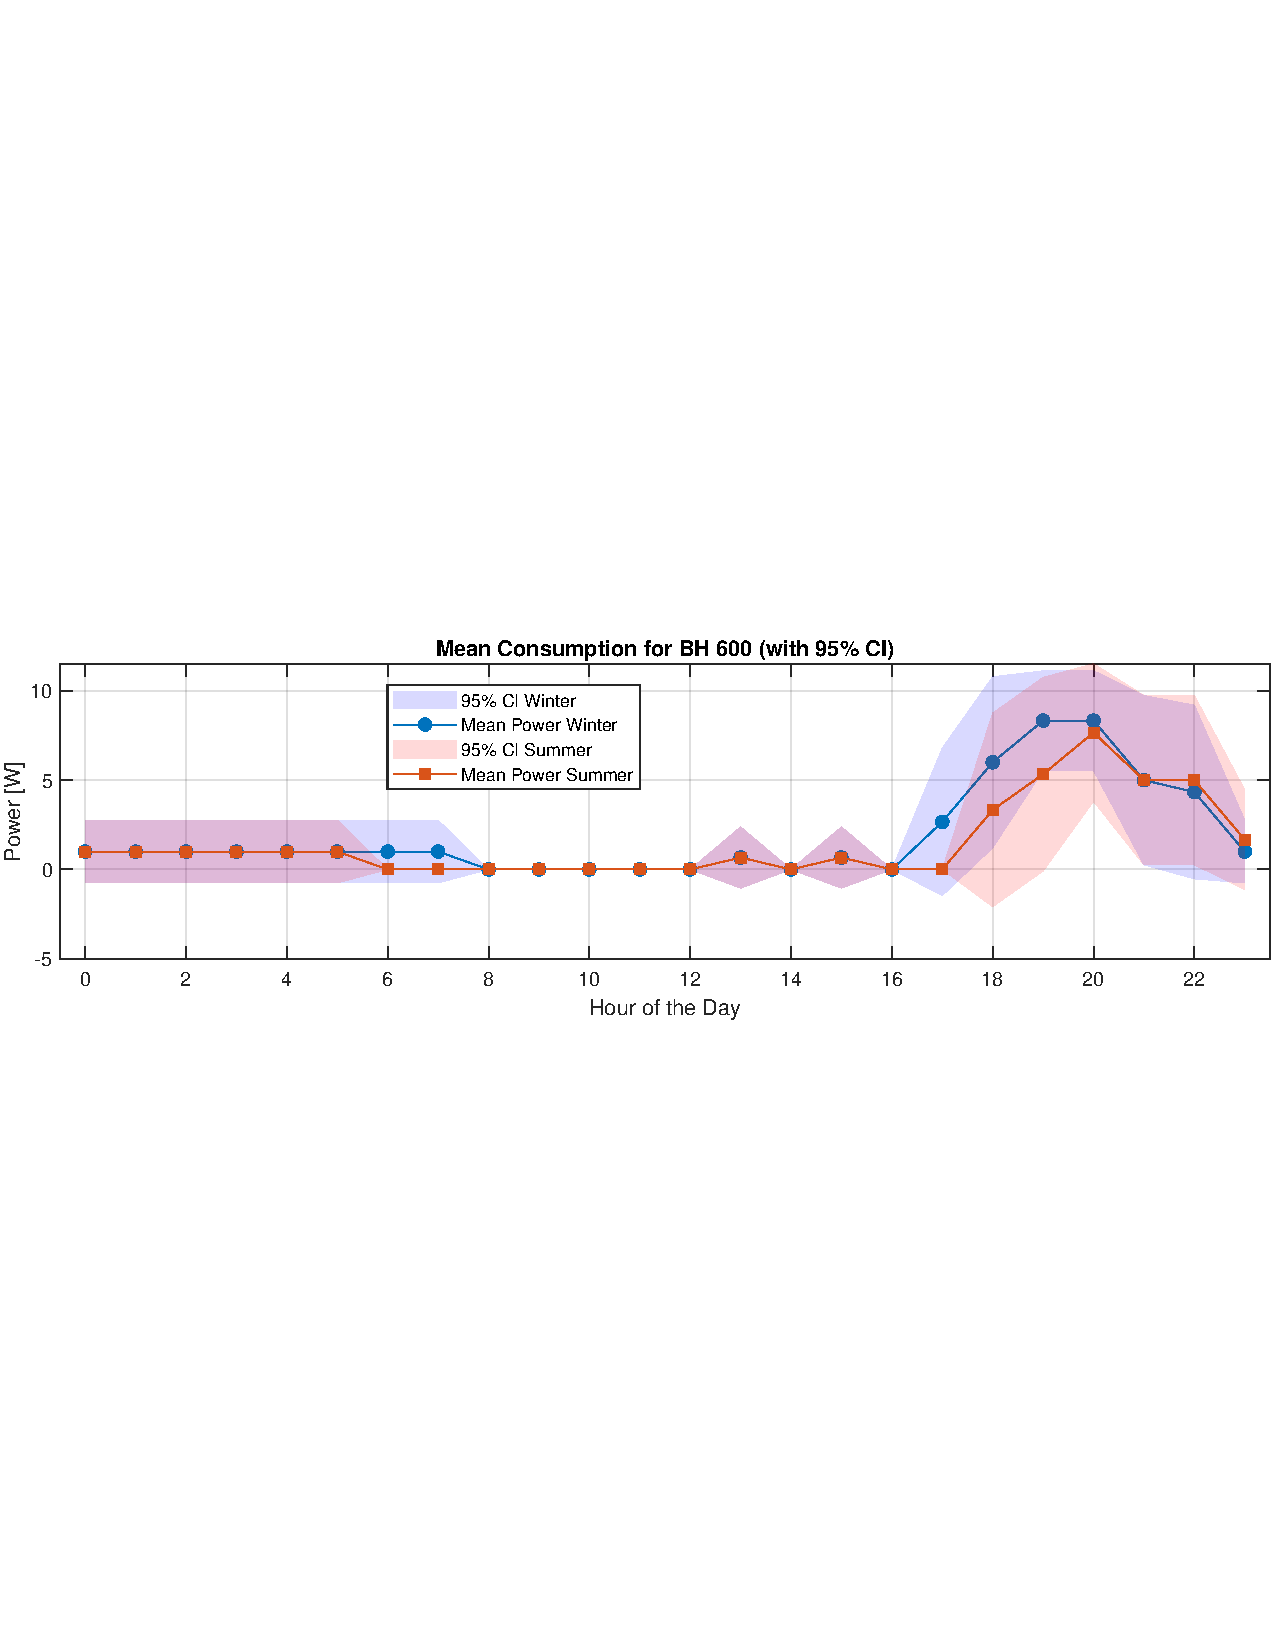
\includegraphics[width=\linewidth, height=\RightImageEachHeight, keepaspectratio]{photos/Mean_consumption_winter&summer_system2_with_95CI.pdf}%\captionsetup{font=tiny}
            %\caption{Consumption for System 2 with CI (Example)}
            %\label{fig:system2_CI}
        \end{subfigure}
        \par\vspace{\RightImageVSpace}
        \begin{subfigure}{\linewidth}
            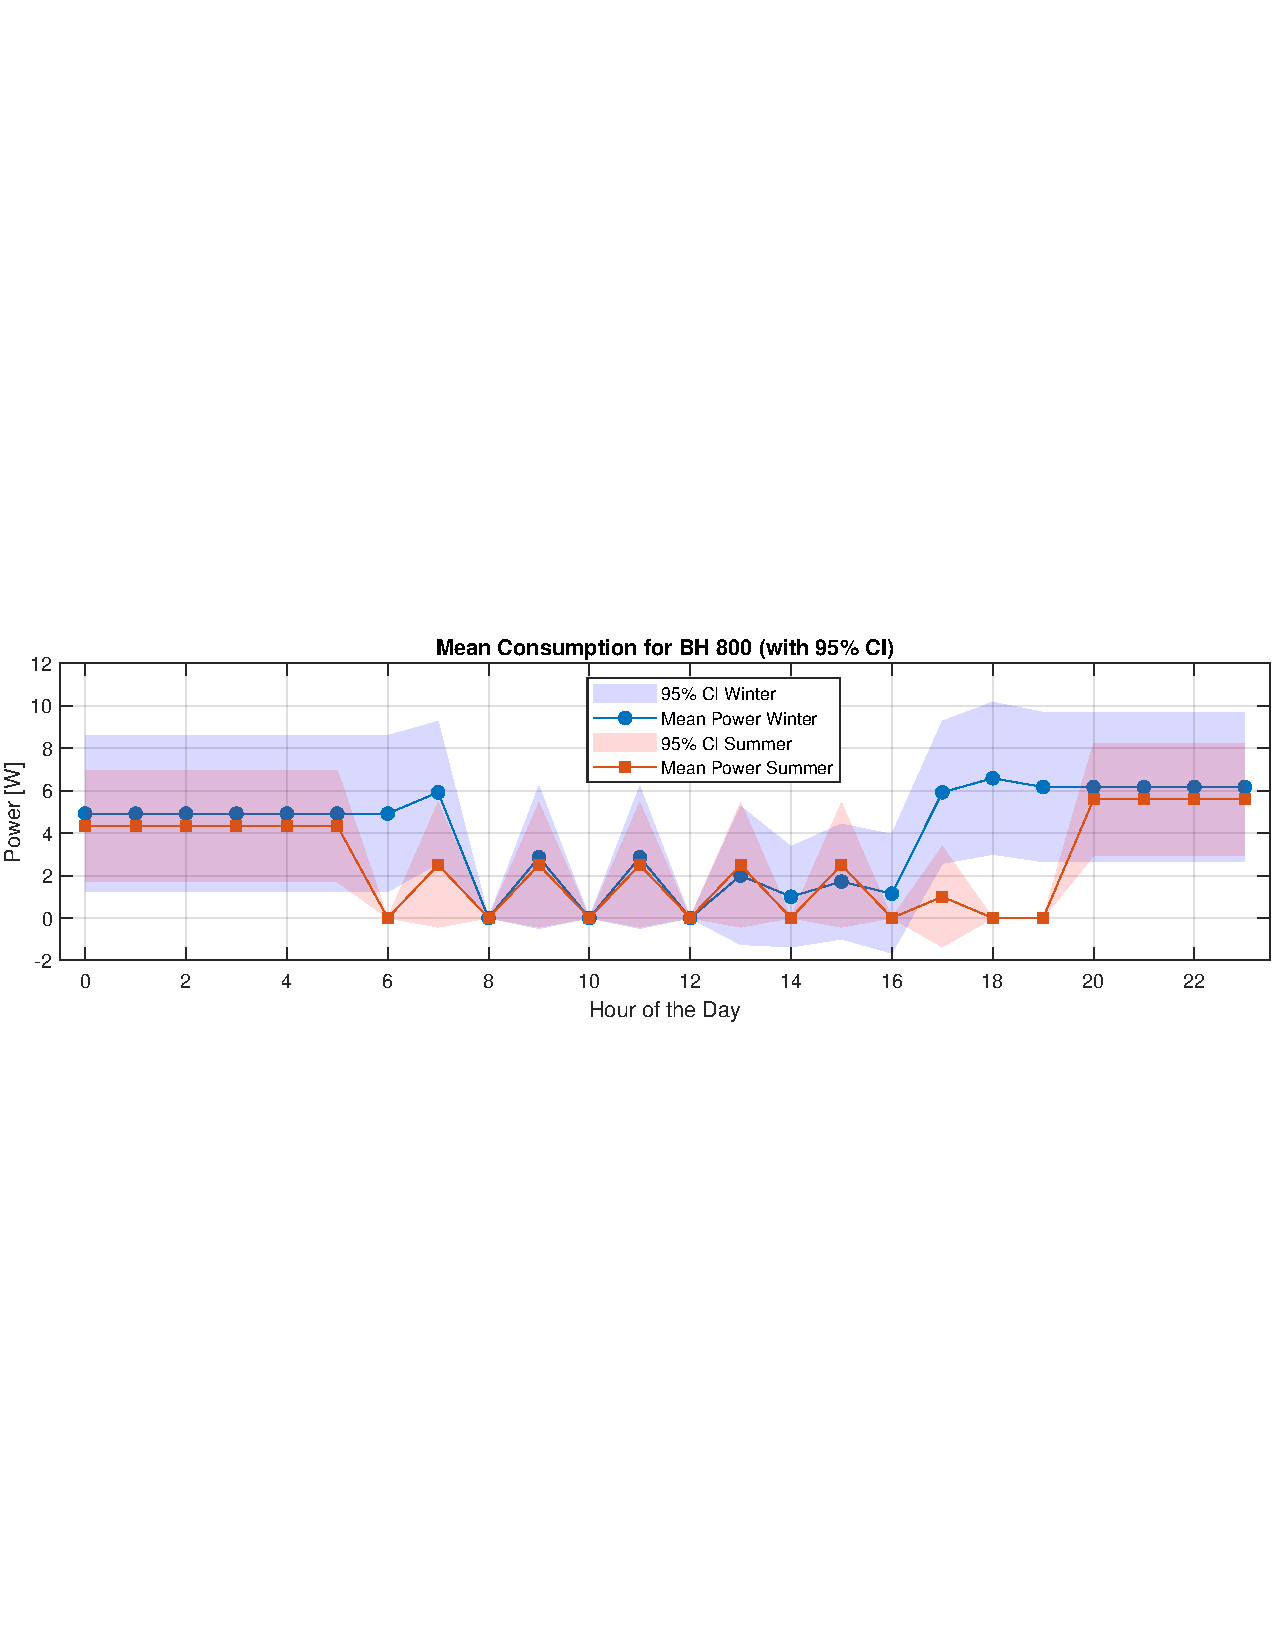
\includegraphics[width=\linewidth, height=\RightImageEachHeight, keepaspectratio]{photos/Mean_consumption_winter&summer_system3_with_95CI.pdf}%\captionsetup{font=tiny}
            %\caption{Consumption for System 3 with CI (Example)}
            %\label{fig:system3_CI}
        \end{subfigure}
    \end{minipage}
    \caption{Mean consumption from all systems during summer and winter. 95\% confidence interval applied. The left figure is for all systems combined with sample size $n=19$, and the right figures are for each system individually. BH 300, BH 600 and BH 800 has respectively $n=5$, $n=6$ and $n=8$ samples.} 
    \label{result:fig:mean_power_allsystems_with95CI}
\end{figure}
Summer and winter mostly differs in regards to when the power peak starts in the evening, and when it stops in the morning. The actual power peak and following consumption pattern matches for both winter and summer data. Using a low sample can give inaccurate data. From figure \ref{result:fig:mean_power_allsystems_with95CI} in the top right for BH 300, we have a small CI for the data. Having a low sample size with no variation, it seems to be more accurate than it is. Using a consumption profile for all of the systems combined may be more accurate, as we can't confirm that the consumption is defined by the size of the system. 

\subsection{General simulations for daily load profile}
In figure \ref{result:fig:Winter_40wpp_all_losses}, we see a simulation of winter data for an 800 system. The data for one day is looped to show how the system will perform over time. From this simulation, we can see that the system is stable with this consumption and production. All loss factors are added in the simulation, to represent a standard system. The \acrfull{soc} drops down to about 0.3 before charging all the way up to 1 in one 24-hour cycle. As long as the SoC hits 1 in a 24-hour cycle, the system will be stable, given there are no sudden changes in production or consumption. Since this is the average of the winter data we can assume that there would be times with worse weather and lower production. Reducing the production would destabilize the cycle over time and empty the battery. 
\begin{figure}[H]
    \centering
    \begin{minipage}[t]{0.655\textwidth} % Adjust width as needed
        \centering
        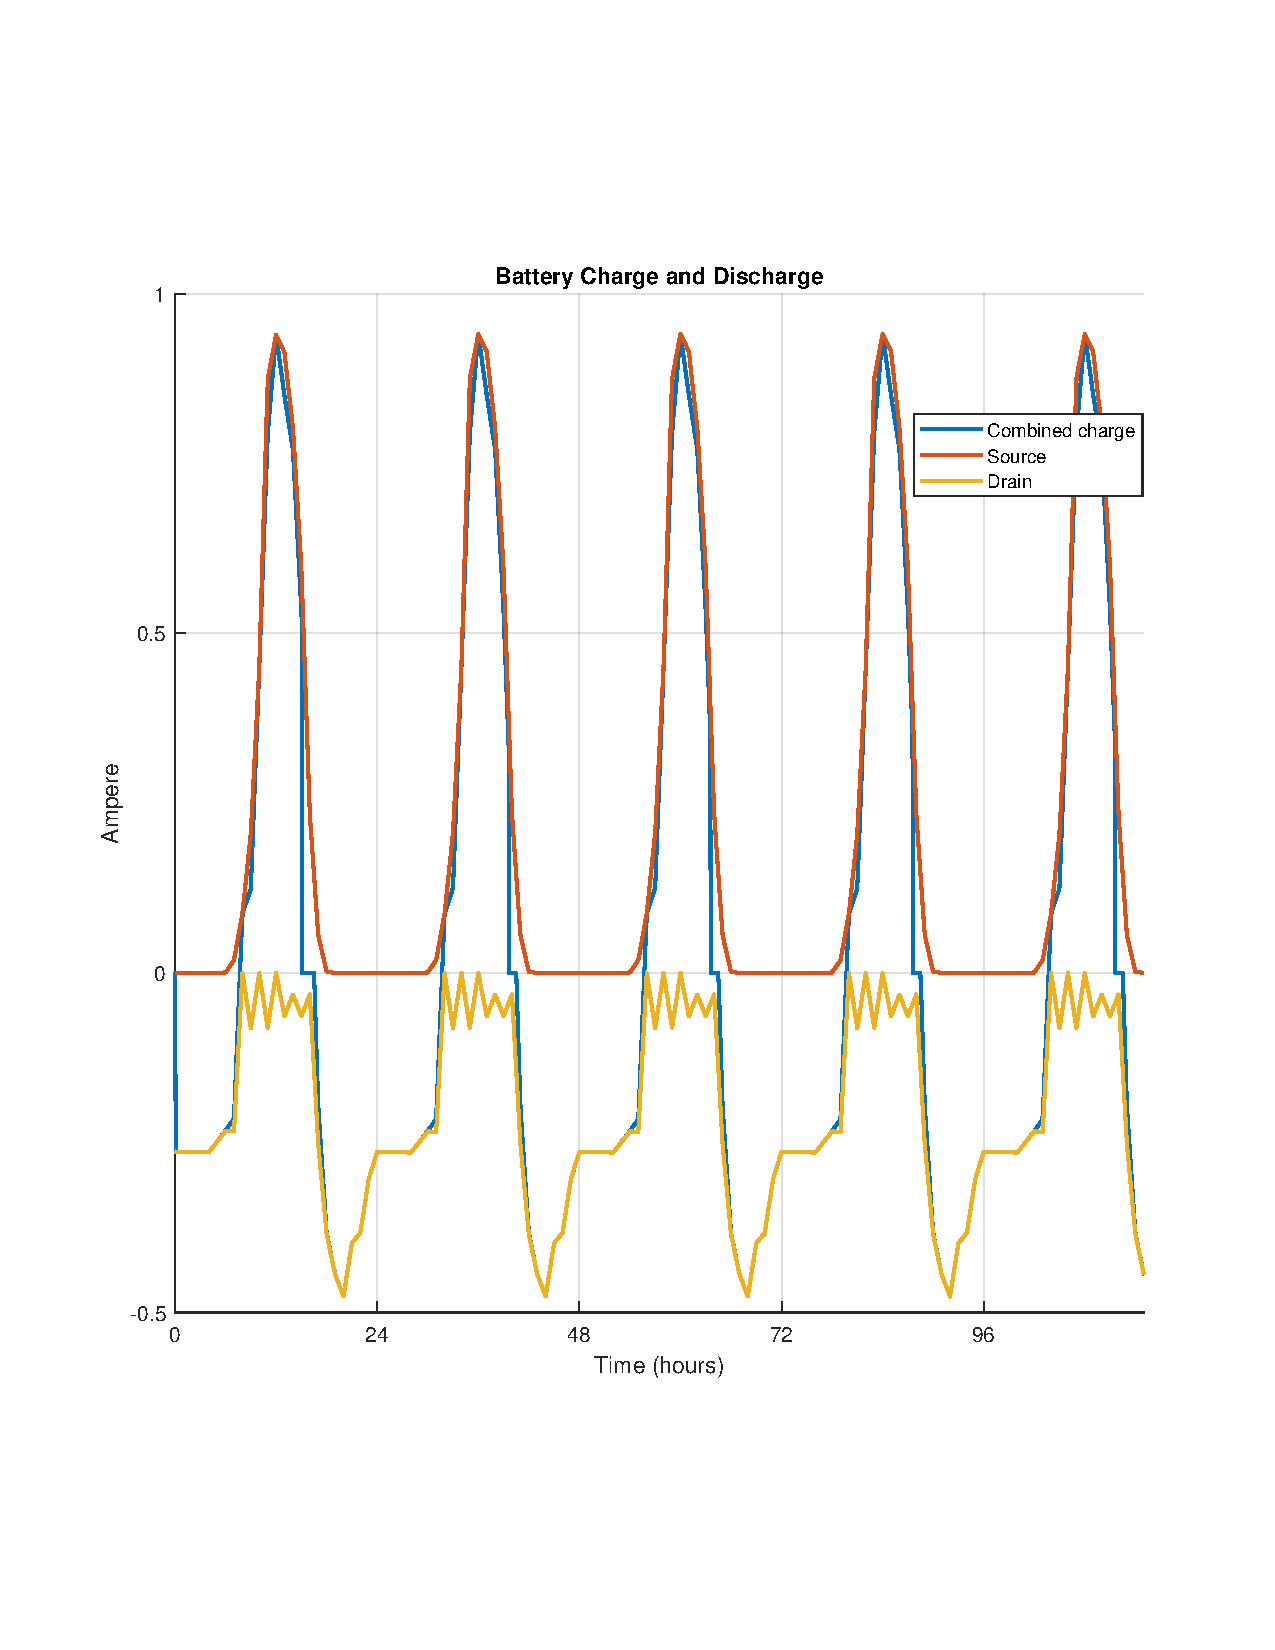
\includegraphics[width=\linewidth]{photos/Winter_charge_with_all_loss_5Days.pdf} %% Gjer denna om til kryss og sirkel
    \end{minipage}%
    \hspace{0.01\textwidth}% Adjust this to control the horizontal space between figure and table
    \begin{minipage}[t]{0.33\textwidth} % Adjust width so (width1 + hspace + width2) is about 1.0\textwidth
        \centering
        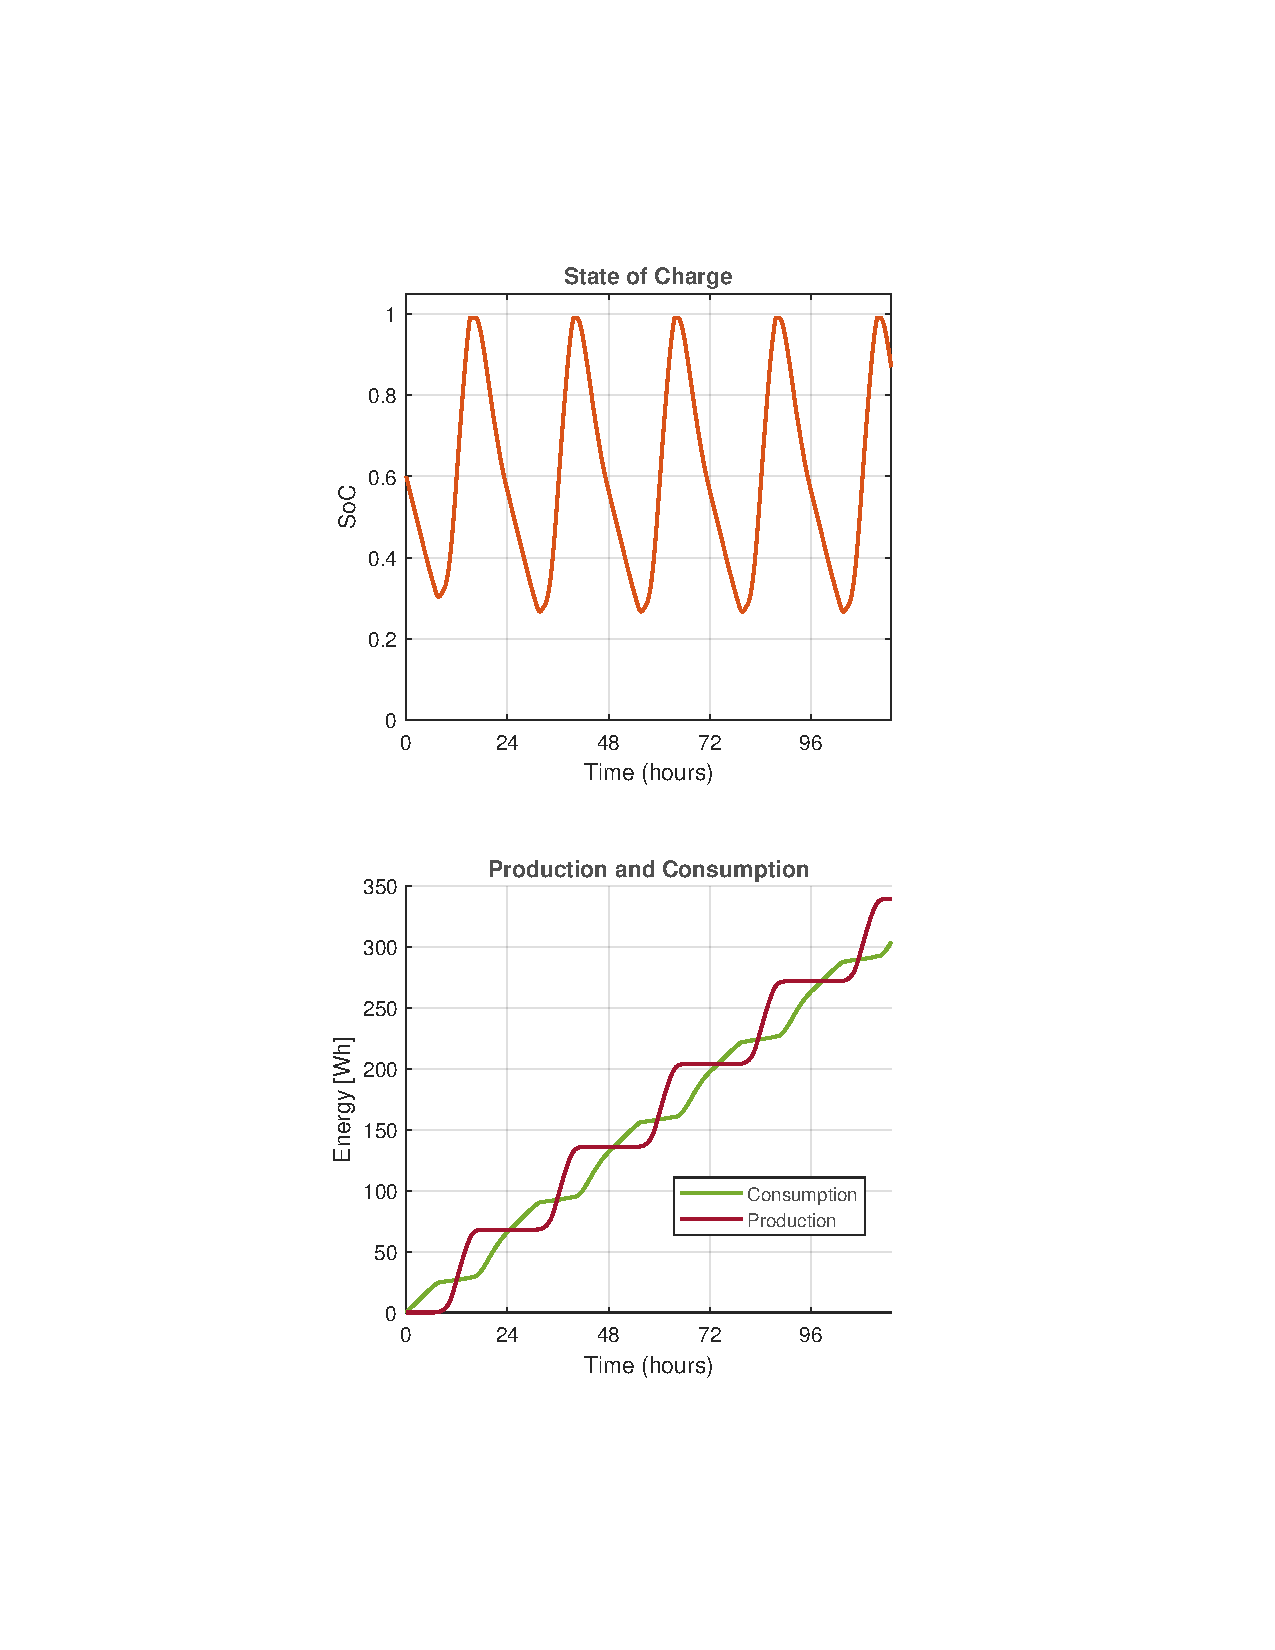
\includegraphics[width=\linewidth]{photos/Winter_SOC&Consumption_with_all_loss_5Days.pdf} %% Gjer denna om til kryss og sirkel
    \end{minipage}
    \captionsetup{font=footnotesize}
    \caption{Winter average production and consumption with all loss factors. Soiling 10\%, general transmission loss 14\% and effectiveness $\eta$ 79\%. The combined charge is the sum of production and consumption. State of charge is the battery charge. Power consumption is integrated from actual usage, and not production. Sample size of consumption profile is $n=19$.}
    \label{result:fig:Winter_40wpp_all_losses}
\end{figure}
The power consumption over five days is about \SI{300}{\watt\hour} of energy. As this cycle is barely stable, the consumption is almost equal to the production. We can see this from the consumption and production lines following each other closely. This gives a good utilization rate in terms of energy usage, using almost all the energy that it produces. 

Figure \ref{result:fig:Summer_40wpp_all_losses} shows a simulation with the summer data. With the increased irradiance in the summer months, this system charges to full each day. With lower consumption than winter, we also have a higher SoC throughout the 24-hour cycle. As seen from the combined charge, the battery stops charging at about peak hours.

\begin{figure}[H]
    \centering
    \begin{minipage}[t]{0.655\textwidth} % Adjust width as needed
        \centering
        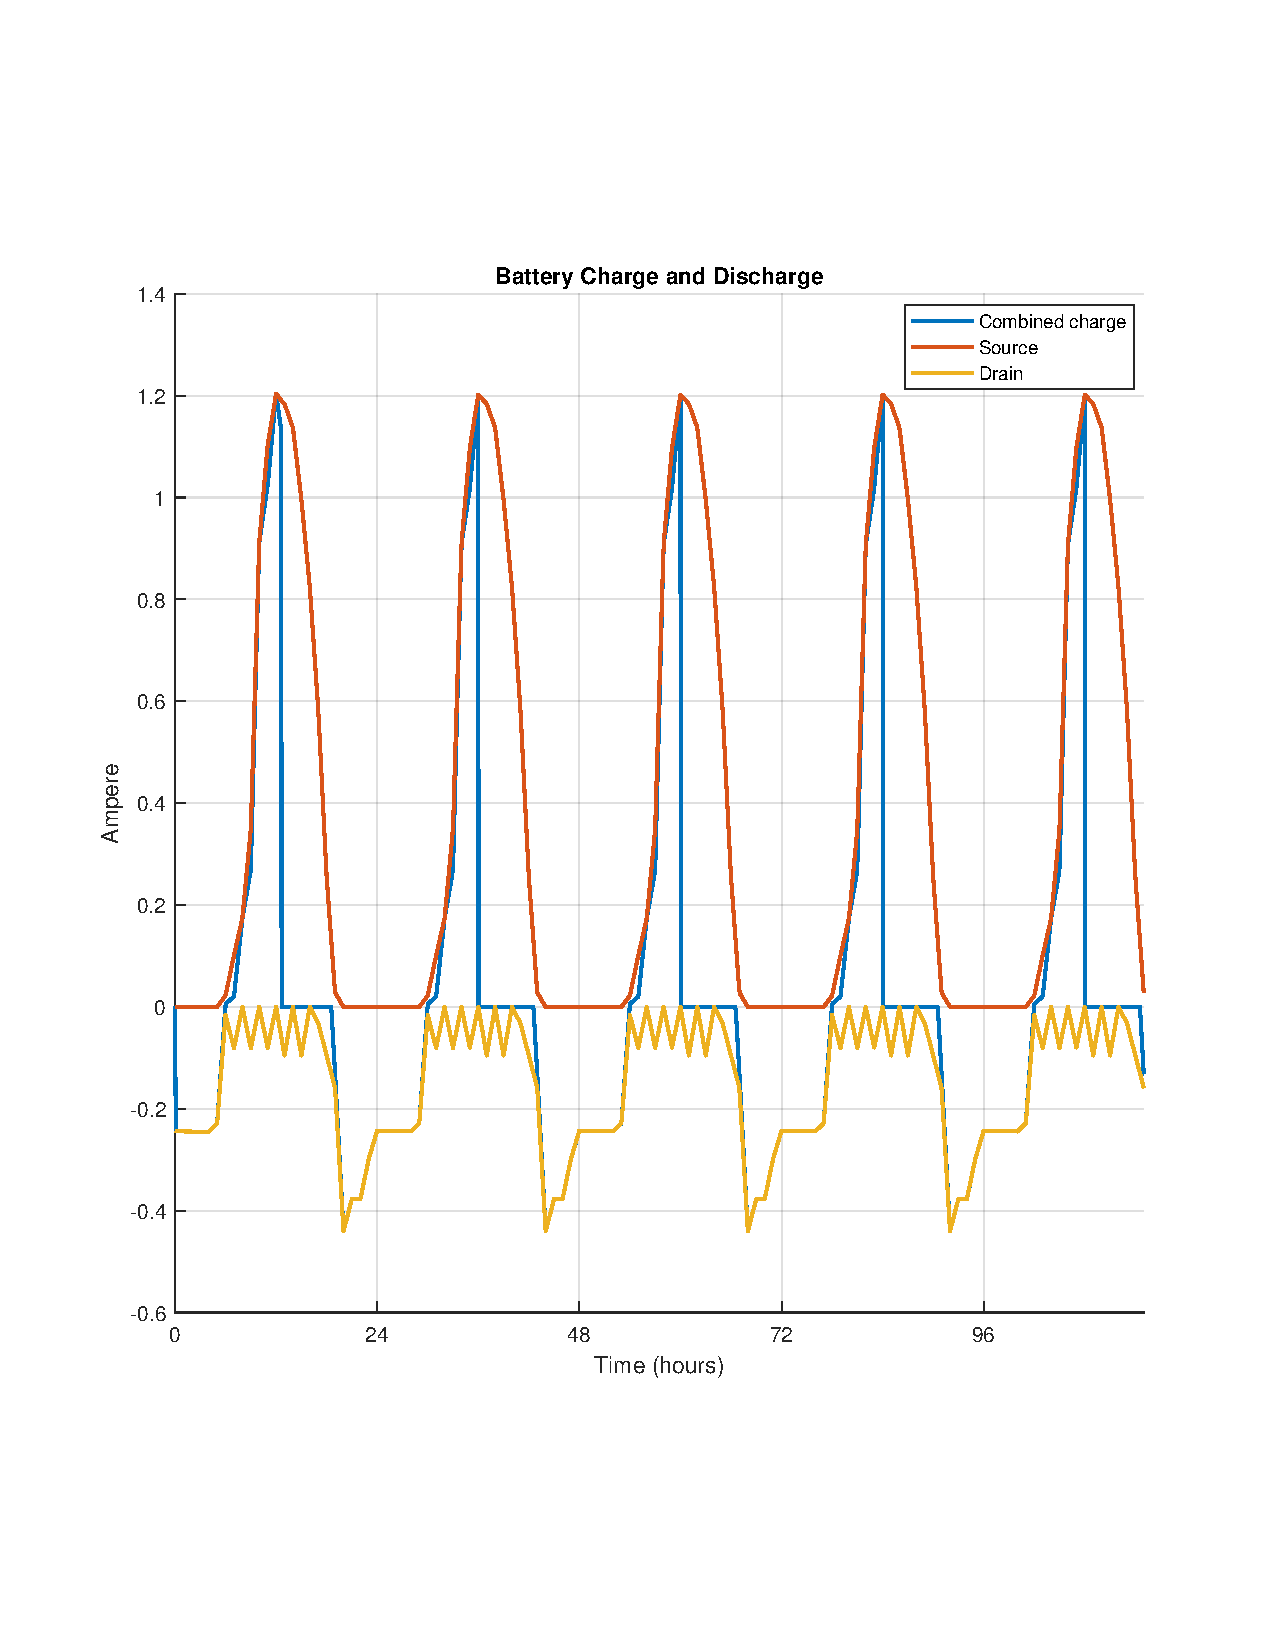
\includegraphics[width=\linewidth]{photos/Summer_charge_with_all_loss_5Days.pdf} %% Gjer denna om til kryss og sirkel
    \end{minipage}%
    \hspace{0.01\textwidth}% Adjust this to control the horizontal space between figure and table
    \begin{minipage}[t]{0.33\textwidth} % Adjust width so (width1 + hspace + width2) is about 1.0\textwidth
        \centering
        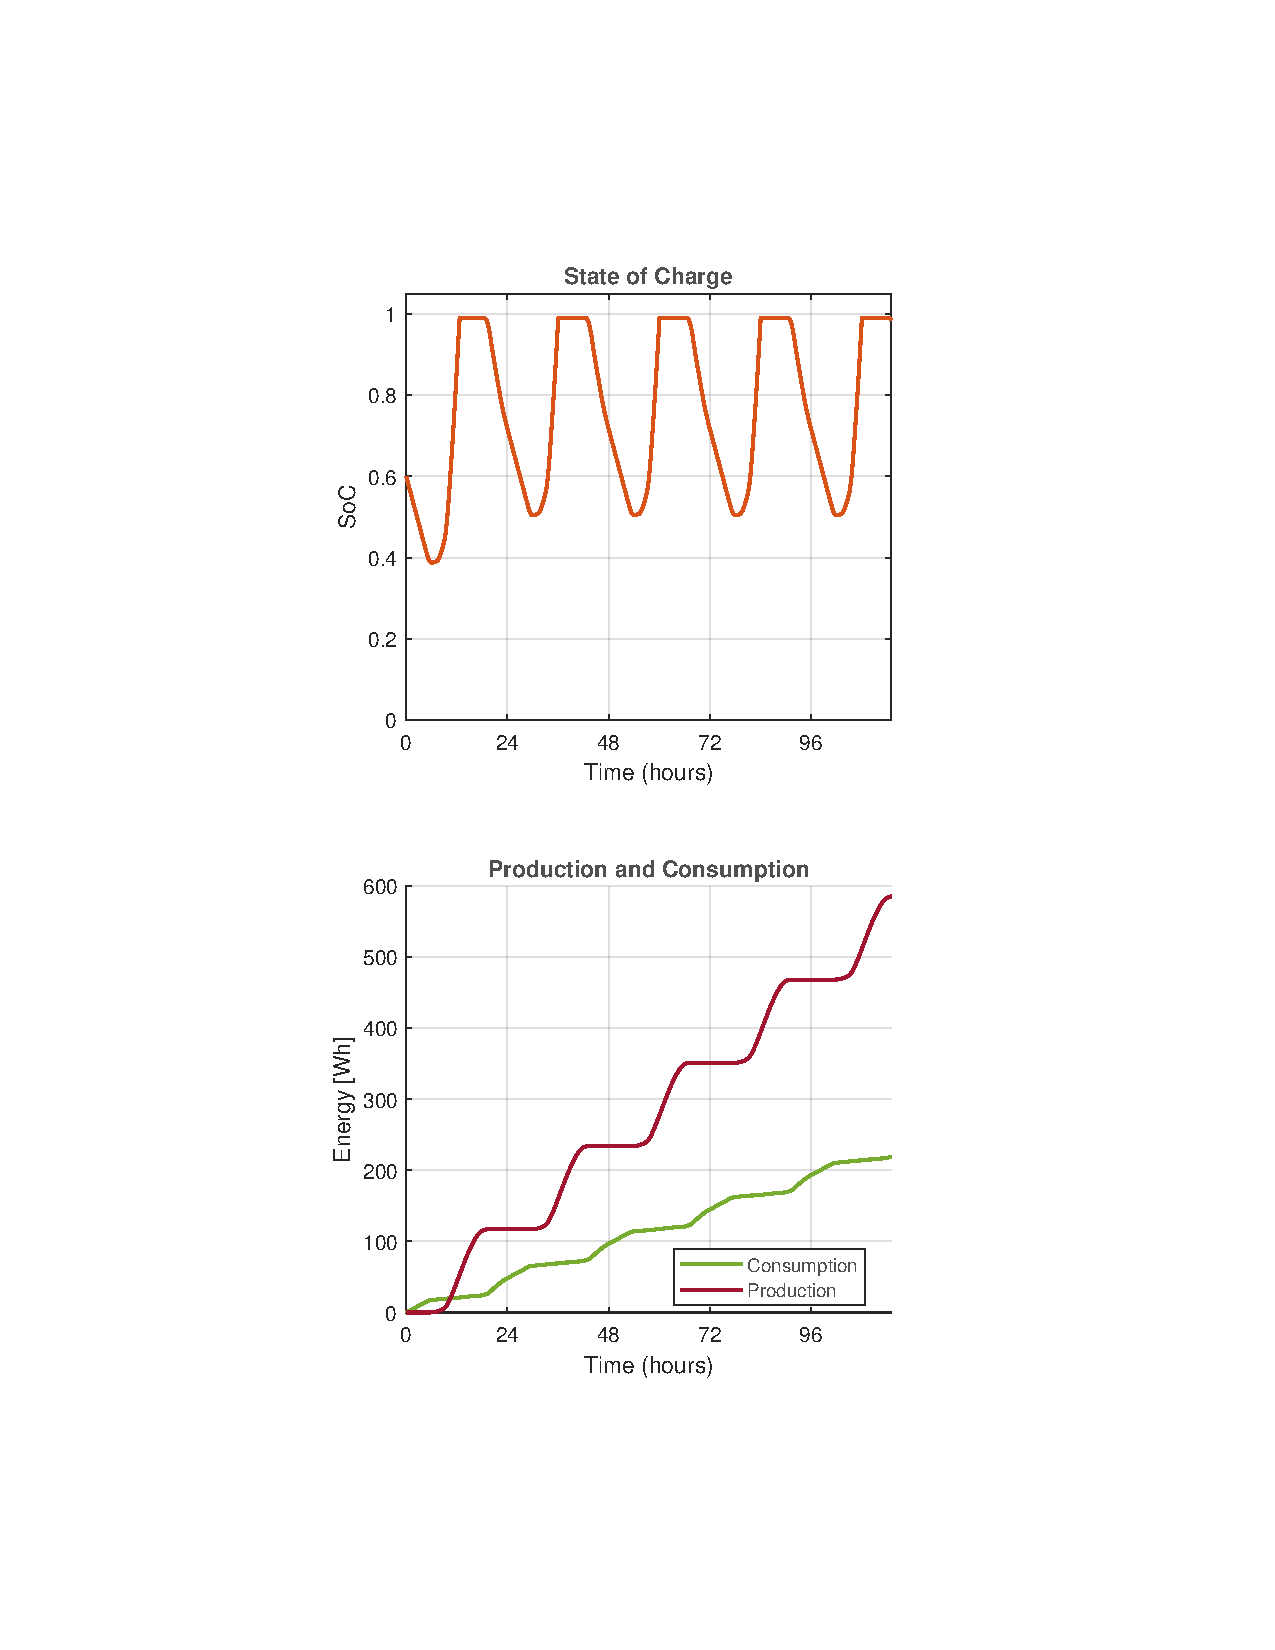
\includegraphics[width=\linewidth]{photos/Summer_SOC&Consumption_with_all_loss_5Days.pdf} %% Gjer denna om til kryss og sirkel
    \end{minipage}
    \captionsetup{font=footnotesize}
    \caption{Summer average production and consumption with all loss factors. Soiling 10\%, general transmission loss 14\% and effectiveness $\eta$ 79\%. The combined charge is the sum of production and consumption. State of charge is the battery charge. Power consumption is integrated from actual usage, and not production. Sample size of consumption profile is $n=19$.}
    \label{result:fig:Summer_40wpp_all_losses}
\end{figure}
Summer production outgrows the consumption, and although we produce almost \SI{600}{\watt\hour} - only about \SI{200}{\watt\hour} is consumed. This gives summer a lower utilization rate than winter. 
\newpage
\subsection{System specific simulations with daily load profile}
\label{sec:systemspesificdata}
\subsubsection{Summer data}
Figures \ref{result:fig:300_summer_soc}, \ref{result:fig:600_summer_soc} and \ref{result:fig:800_summer_soc} show the systems when compared towards the system specific consumption data. All loss factors are included. When using this setup, we risk having a small sample size for the consumption profile. 
\begin{minipage}[t]{0.32\textwidth} % Adjust width as needed
    \begin{figure}[H]
        \centering
        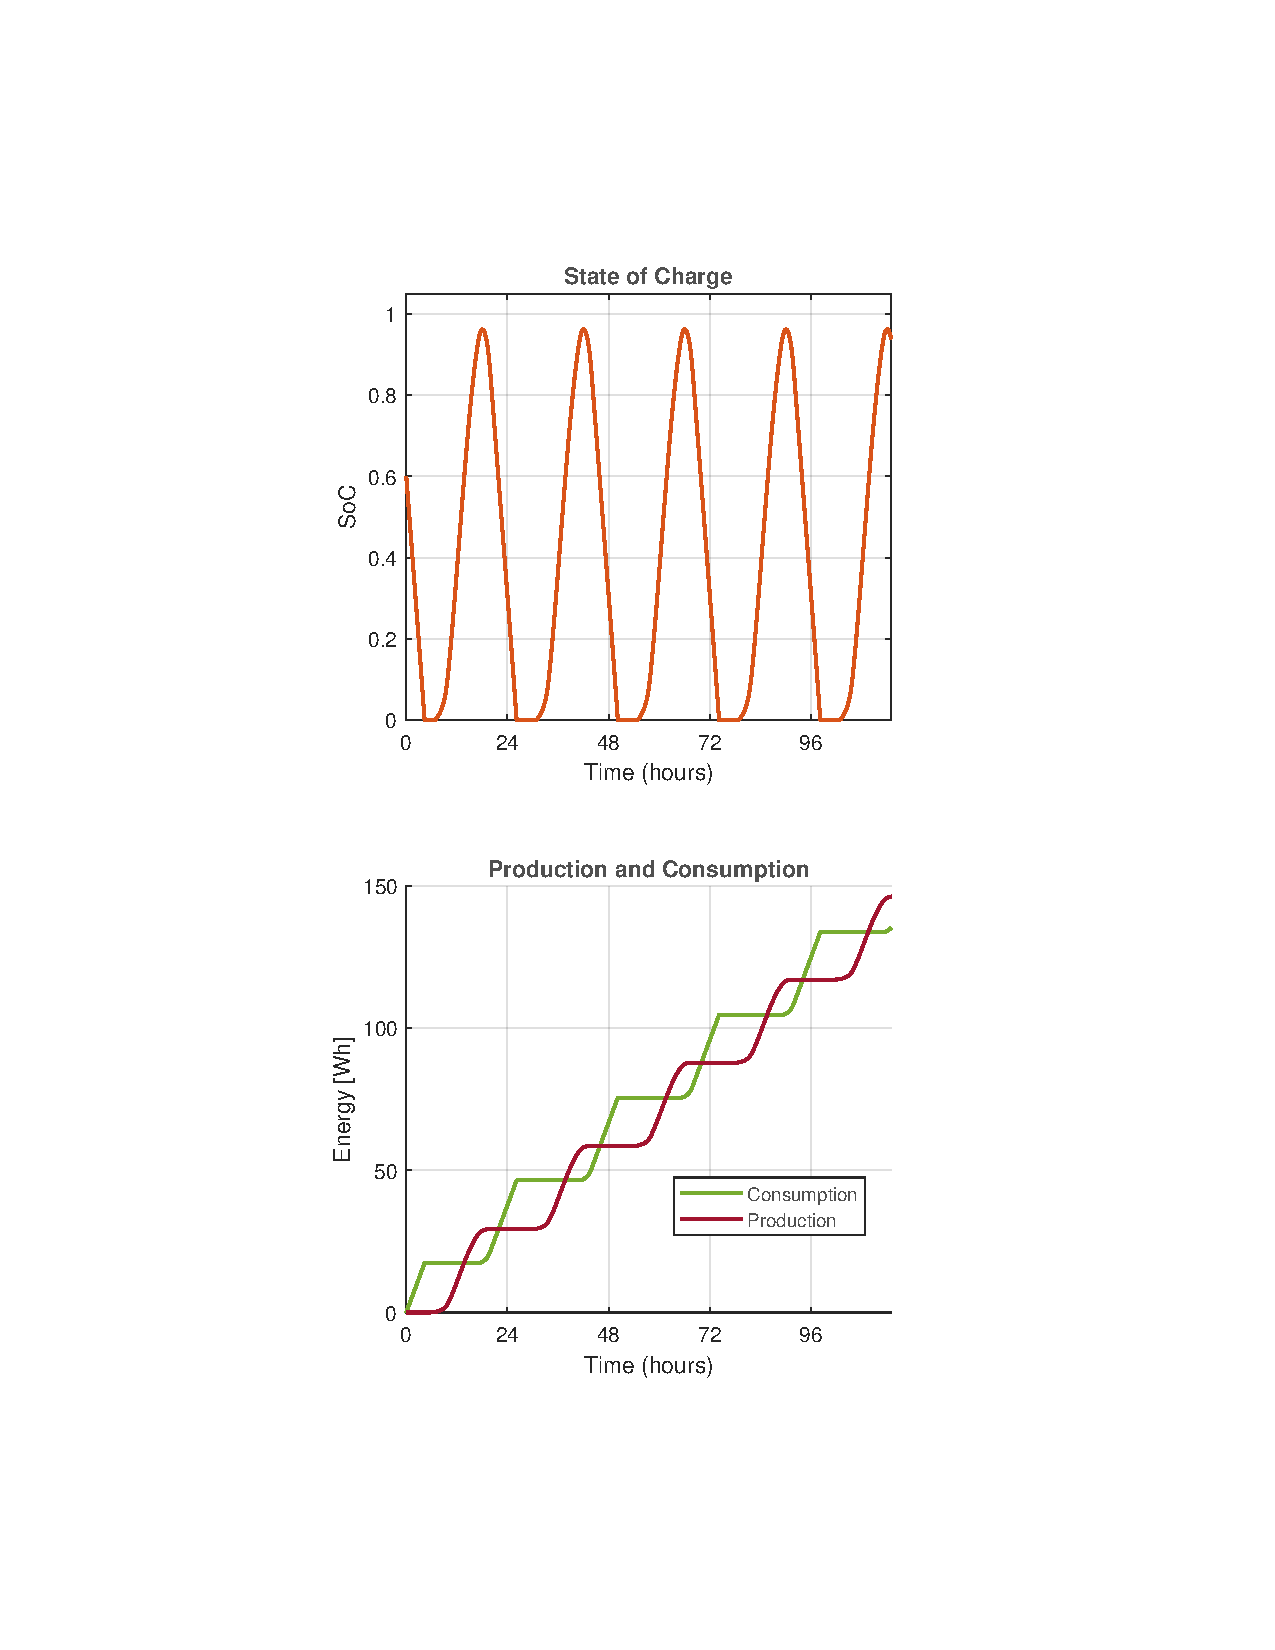
\includegraphics[width=\linewidth]{photos/Summer_SOC&Consumption_with_all_loss_5Days_300System.pdf} %% Gjer denna om til kryss og sirkel
        \captionsetup{font=footnotesize} % Or footnotesize, etc
        \caption{BH 300 System SoC, production and consumption for summer data. Soiling 10\%, general transmission loss 14\% and effectiveness $\eta$ 79\%.}
        \label{result:fig:300_summer_soc}
    \end{figure}
\end{minipage}% <--- IMPORTANT: The '%' symbol prevents unwanted horizontal space
\hspace{0.02\textwidth}% Adjust this to control the horizontal space between figure and table
\begin{minipage}[t]{0.32\textwidth} % Adjust width so (width1 + hspace + width2) is about 1.0\textwidth
    \begin{figure}[H]
        \centering
        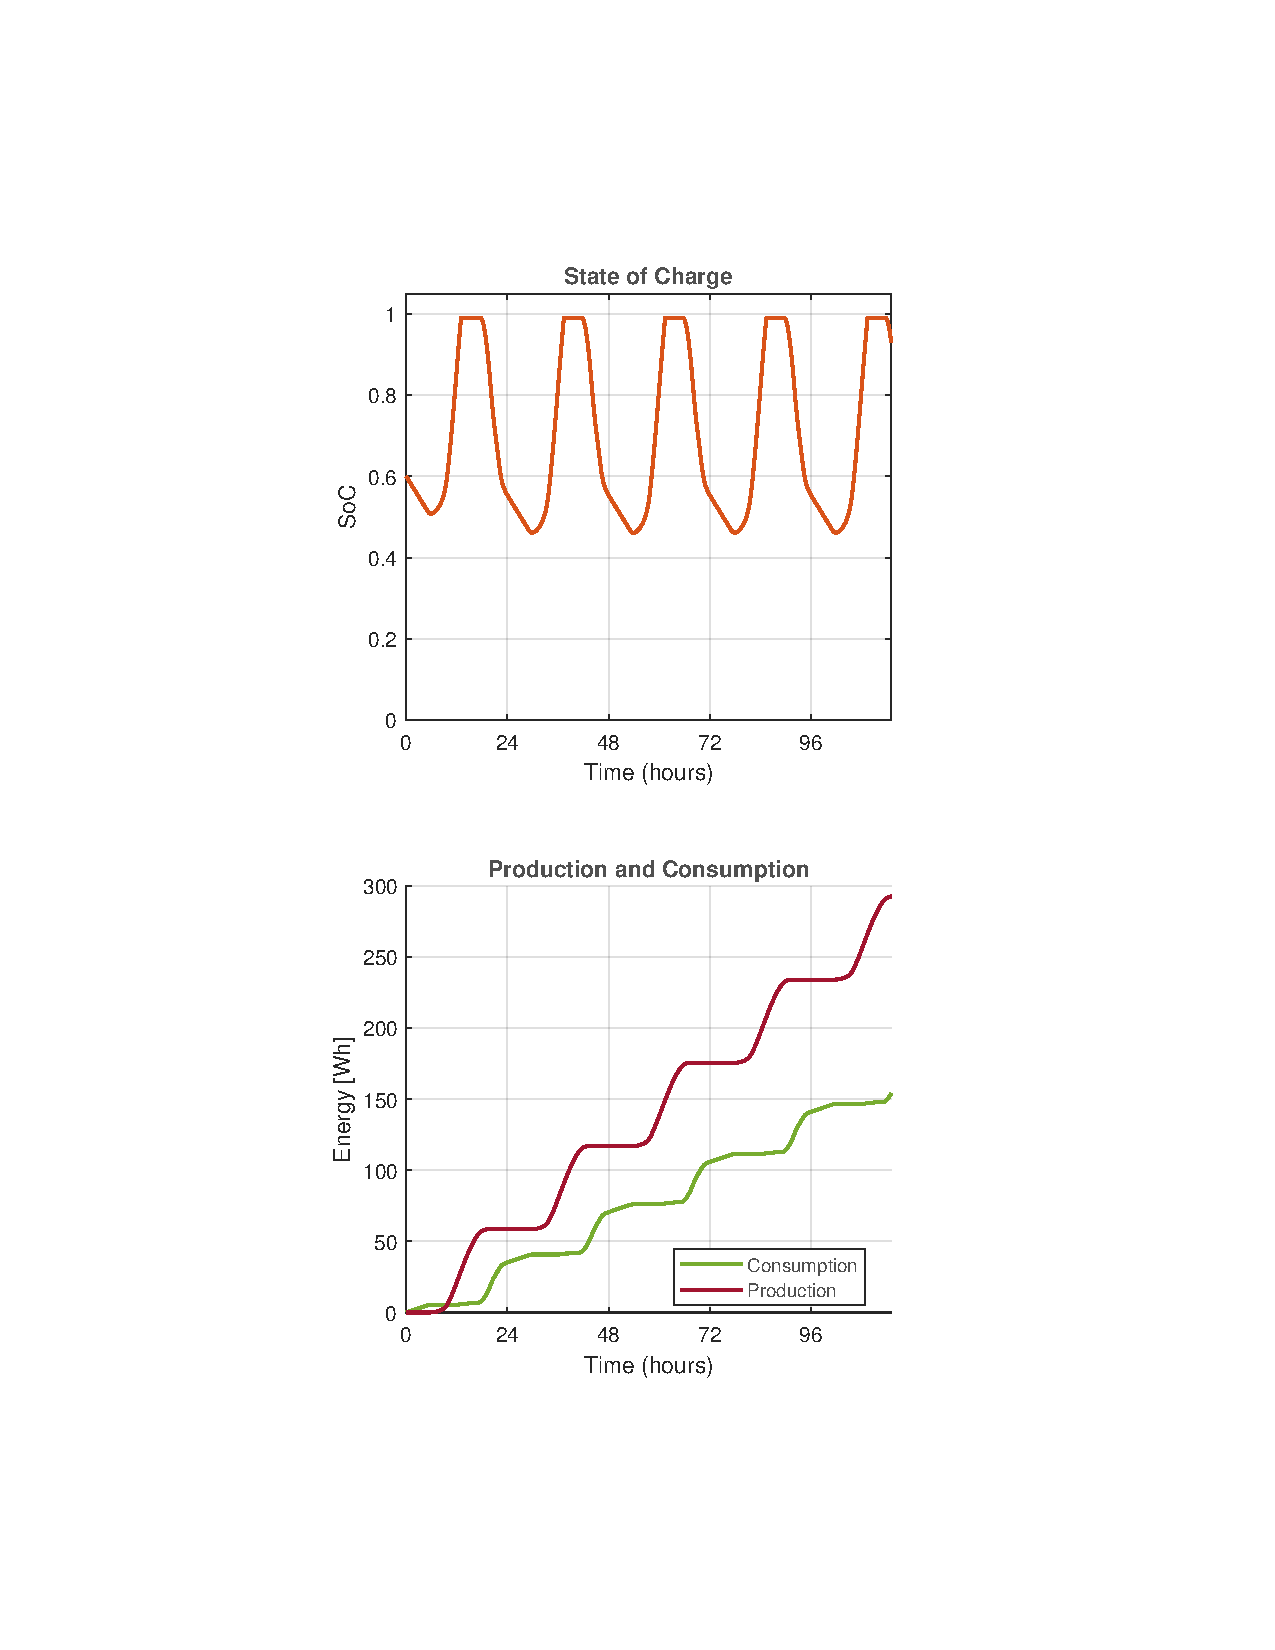
\includegraphics[width=\linewidth]{photos/Summer_SOC&Consumption_with_all_loss_5Days_600System.pdf} %% Gjer denna om til kryss og sirkel
        \captionsetup{font=footnotesize} % Or footnotesize, etc
        \caption{BH 600 System SoC, production and consumption for summer data. Soiling 10\%, general transmission loss 14\% and effectiveness $\eta$ 79\%.}
        \label{result:fig:600_summer_soc}
    \end{figure}
\end{minipage}
\hspace{0.02\textwidth}% Adjust this to control the horizontal space between figure and table
\begin{minipage}[t]{0.32\textwidth} % Adjust width so (width1 + hspace + width2) is about 1.0\textwidth
    \begin{figure}[H]
        \centering
        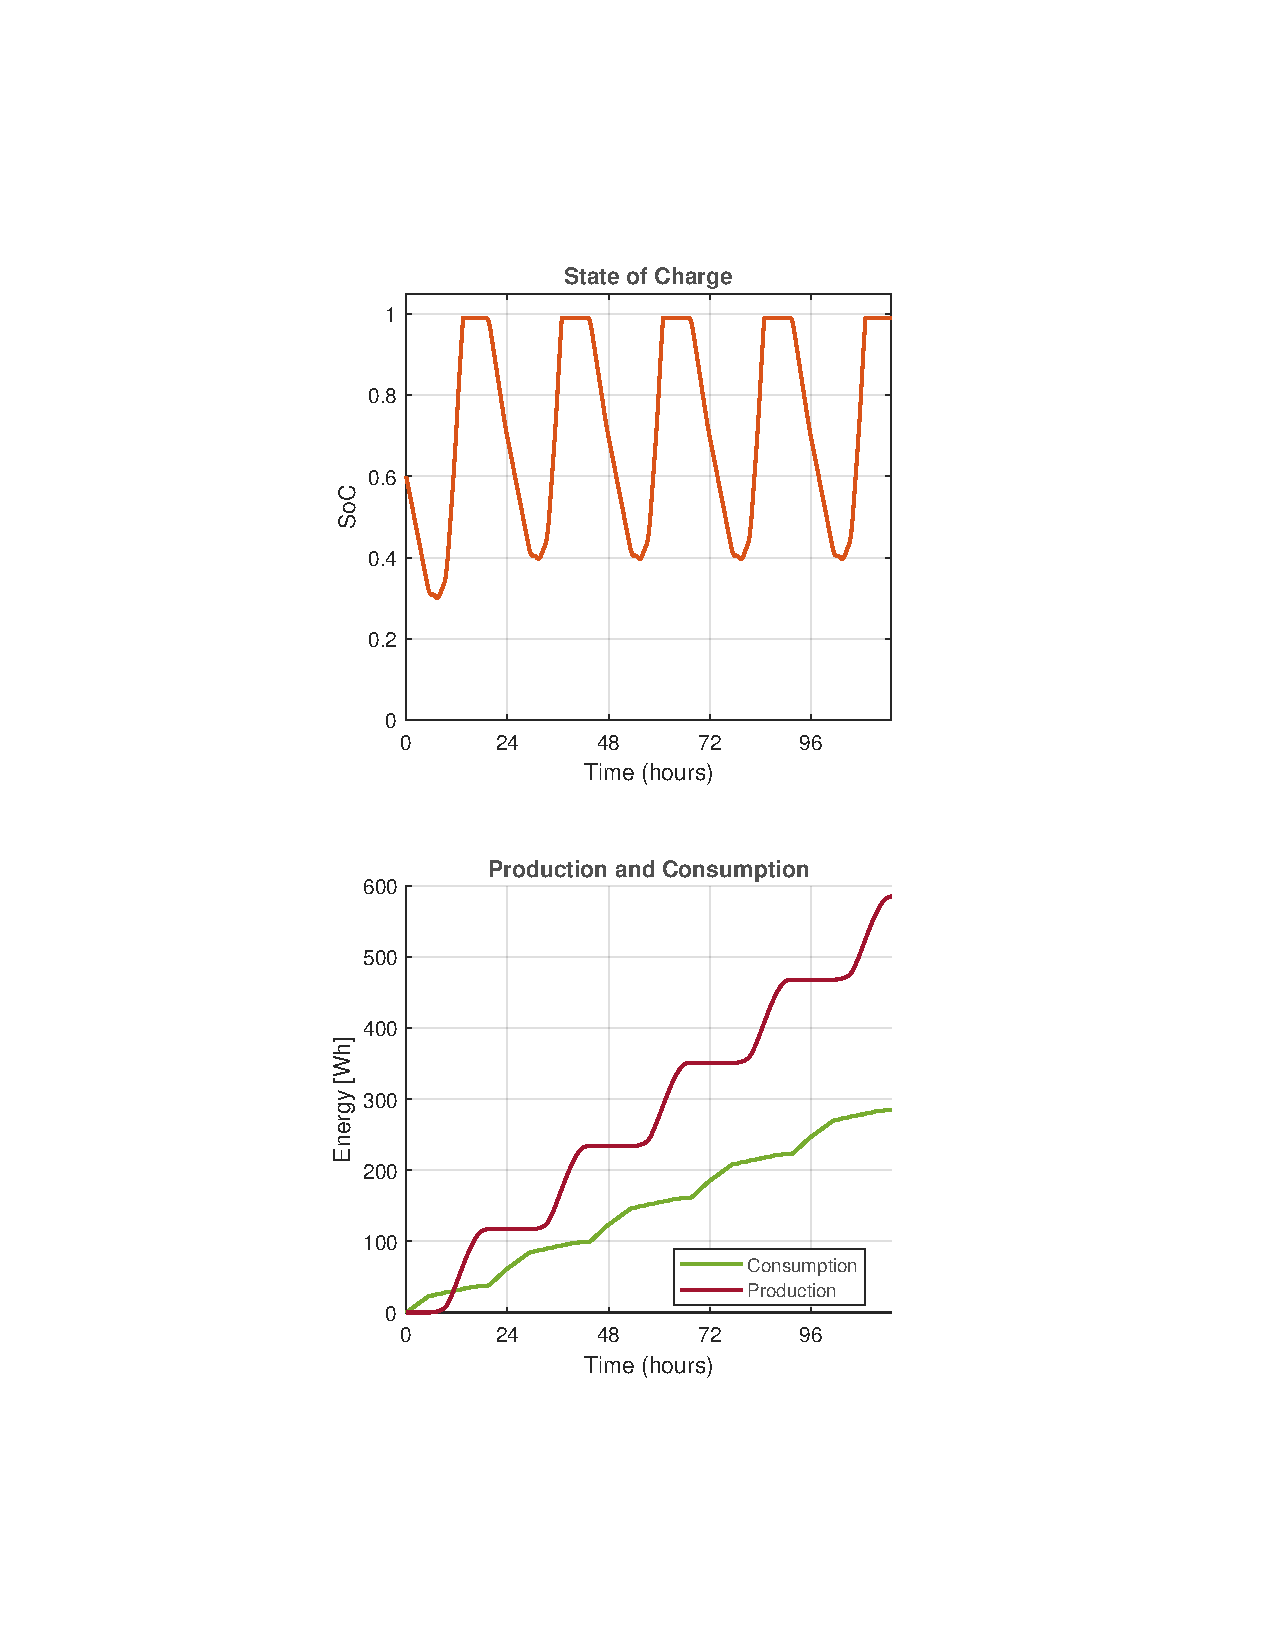
\includegraphics[width=\linewidth]{photos/Summer_SOC&Consumption_with_all_loss_5Days_800System.pdf} %% Gjer denna om til kryss og sirkel
        \captionsetup{font=footnotesize} % Or footnotesize, etc.
        \caption{BH 800 System SoC, production and consumption for summer data. Soiling 10\%, general transmission loss 14\% and effectiveness $\eta$ 79\%.}
        \label{result:fig:800_summer_soc}
    \end{figure}
\end{minipage}

Firstly we can see the difference in the consumption from the systems. BH 300 will consume at 140Wh, BH 600 will consume 150Wh, and BH 800 will consume 300Wh. We can also see the difference in the SoC, where the BH 300 will completely empty itself and almost receive a full charge in one day. For difference, the BH 600 and BH 800 will only use about half of their battery capacity. As this is during the summer months, we can assume a grater amplitude in the winter months. 
\newpage
\subsubsection{Winter data}
On figures \ref{result:fig:300_winter_soc}, \ref{result:fig:600_winter_soc} and \ref{result:fig:800_winter_soc} we can see the winter results with the same setup as the summer data. All loss factors are included.
\begin{minipage}[t]{0.32\textwidth} % Adjust width as needed
    \begin{figure}[H]
        \centering
        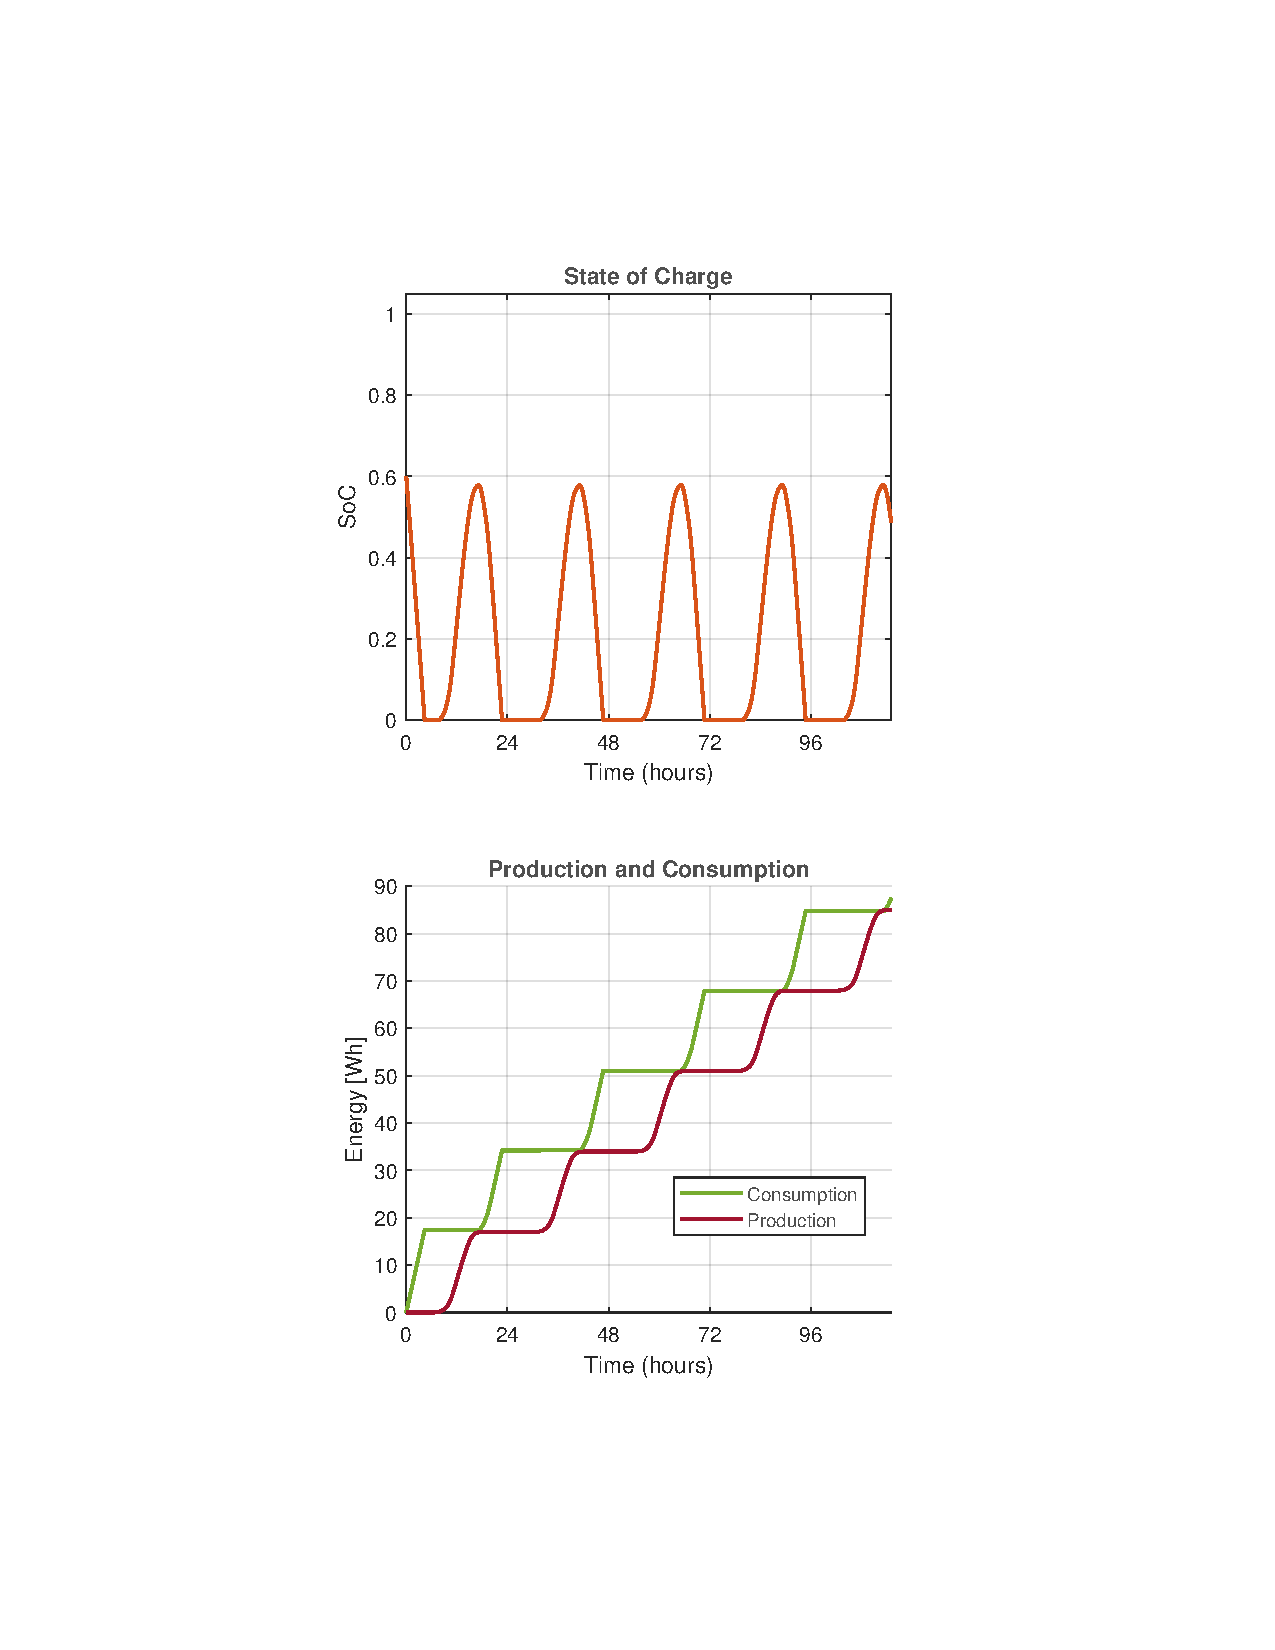
\includegraphics[width=\linewidth]{photos/Winter_SOC&Consumption_with_all_loss_5Days_300System.pdf} %% Gjer denna om til kryss og sirkel
        \captionsetup{font=footnotesize} % Or footnotesize, etc
        \caption{BH 300 System SoC, production and consumption for winter data. Soiling 10\%, general transmission loss 14\% and effectiveness $\eta$ 79\%.}
        \label{result:fig:300_winter_soc}
    \end{figure}
\end{minipage}% <--- IMPORTANT: The '%' symbol prevents unwanted horizontal space
\hspace{0.02\textwidth}% Adjust this to control the horizontal space between figure and table
\begin{minipage}[t]{0.32\textwidth} % Adjust width so (width1 + hspace + width2) is about 1.0\textwidth
    \begin{figure}[H]
        \centering
        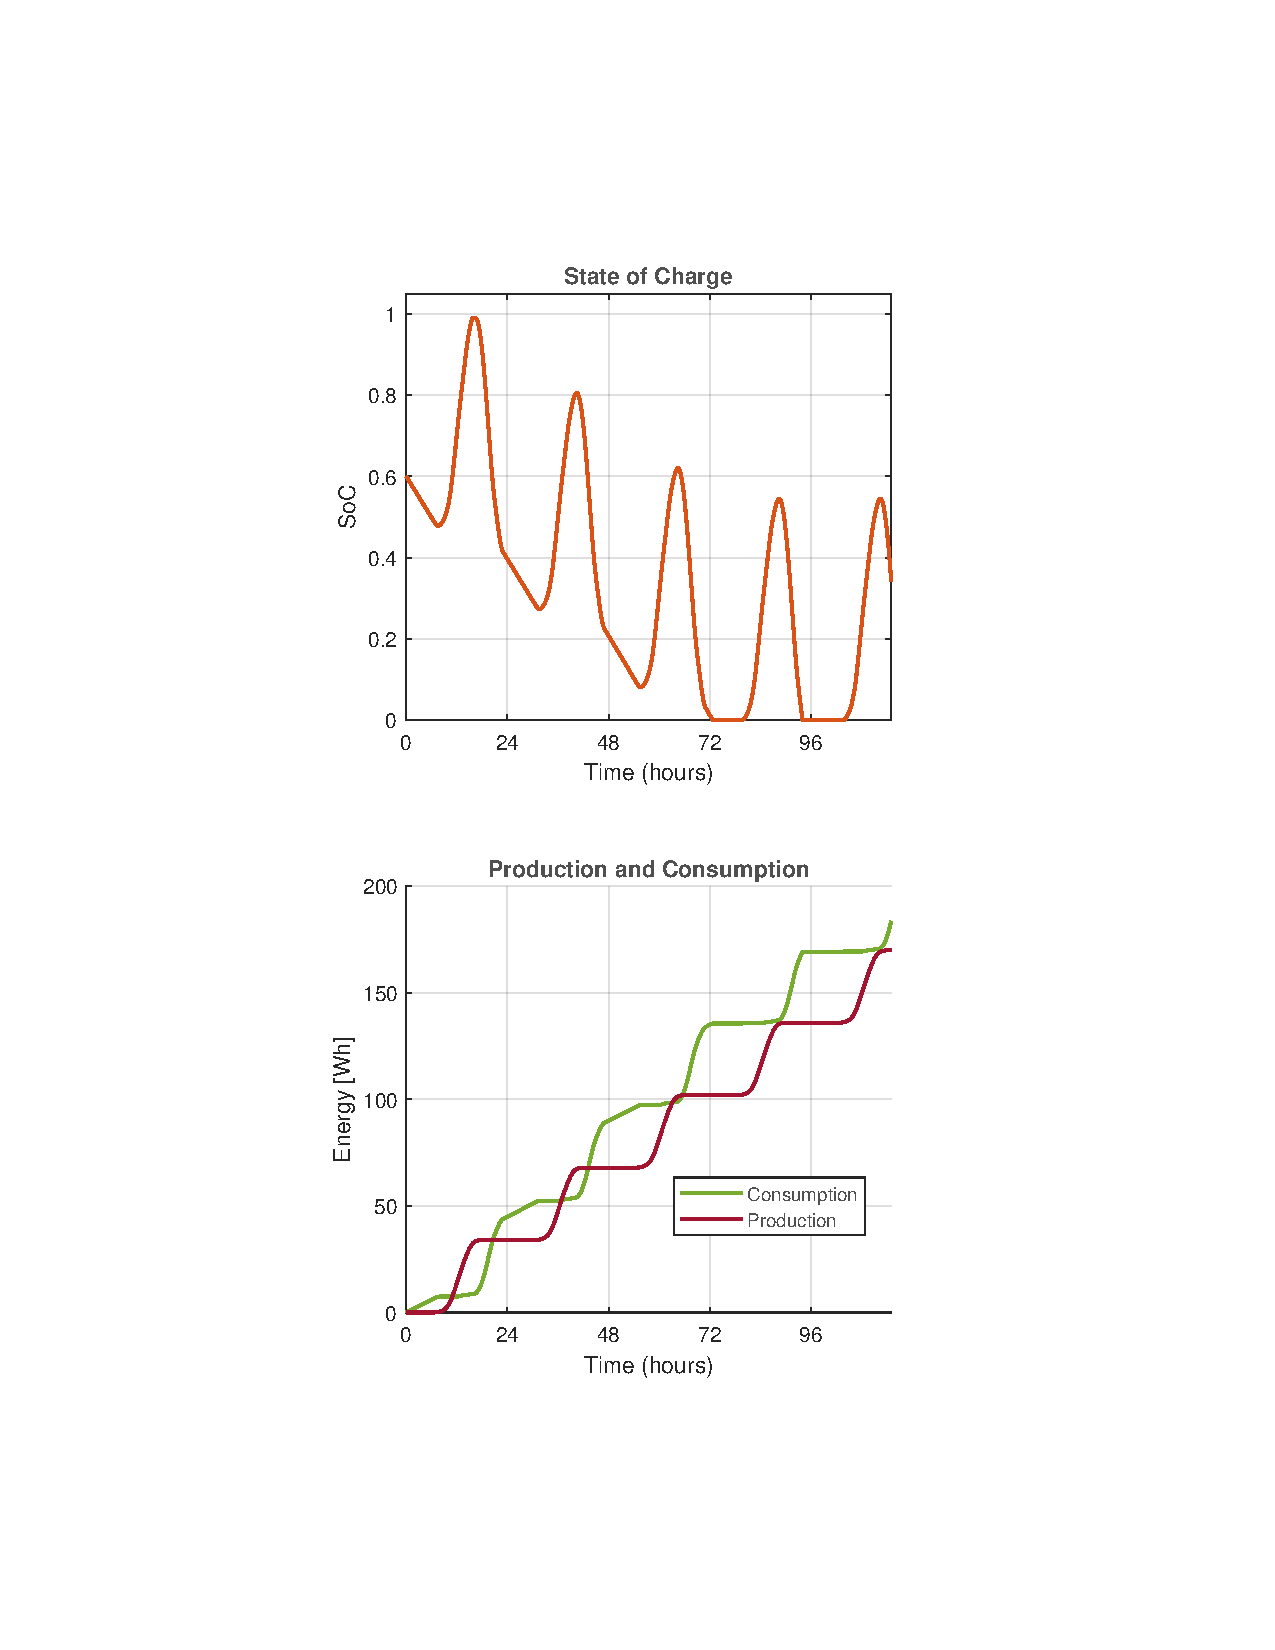
\includegraphics[width=\linewidth]{photos/Winter_SOC&Consumption_with_all_loss_5Days_600System.pdf} %% Gjer denna om til kryss og sirkel
        \captionsetup{font=footnotesize} % Or footnotesize, etc
        \caption{BH 600 System SoC, production and consumption for winter data. Soiling 10\%, general transmission loss 14\% and effectiveness $\eta$ 79\%.}
        \label{result:fig:600_winter_soc}
    \end{figure}
\end{minipage}
\hspace{0.02\textwidth}% Adjust this to control the horizontal space between figure and table
\begin{minipage}[t]{0.32\textwidth} % Adjust width so (width1 + hspace + width2) is about 1.0\textwidth
    \begin{figure}[H]
        \centering
        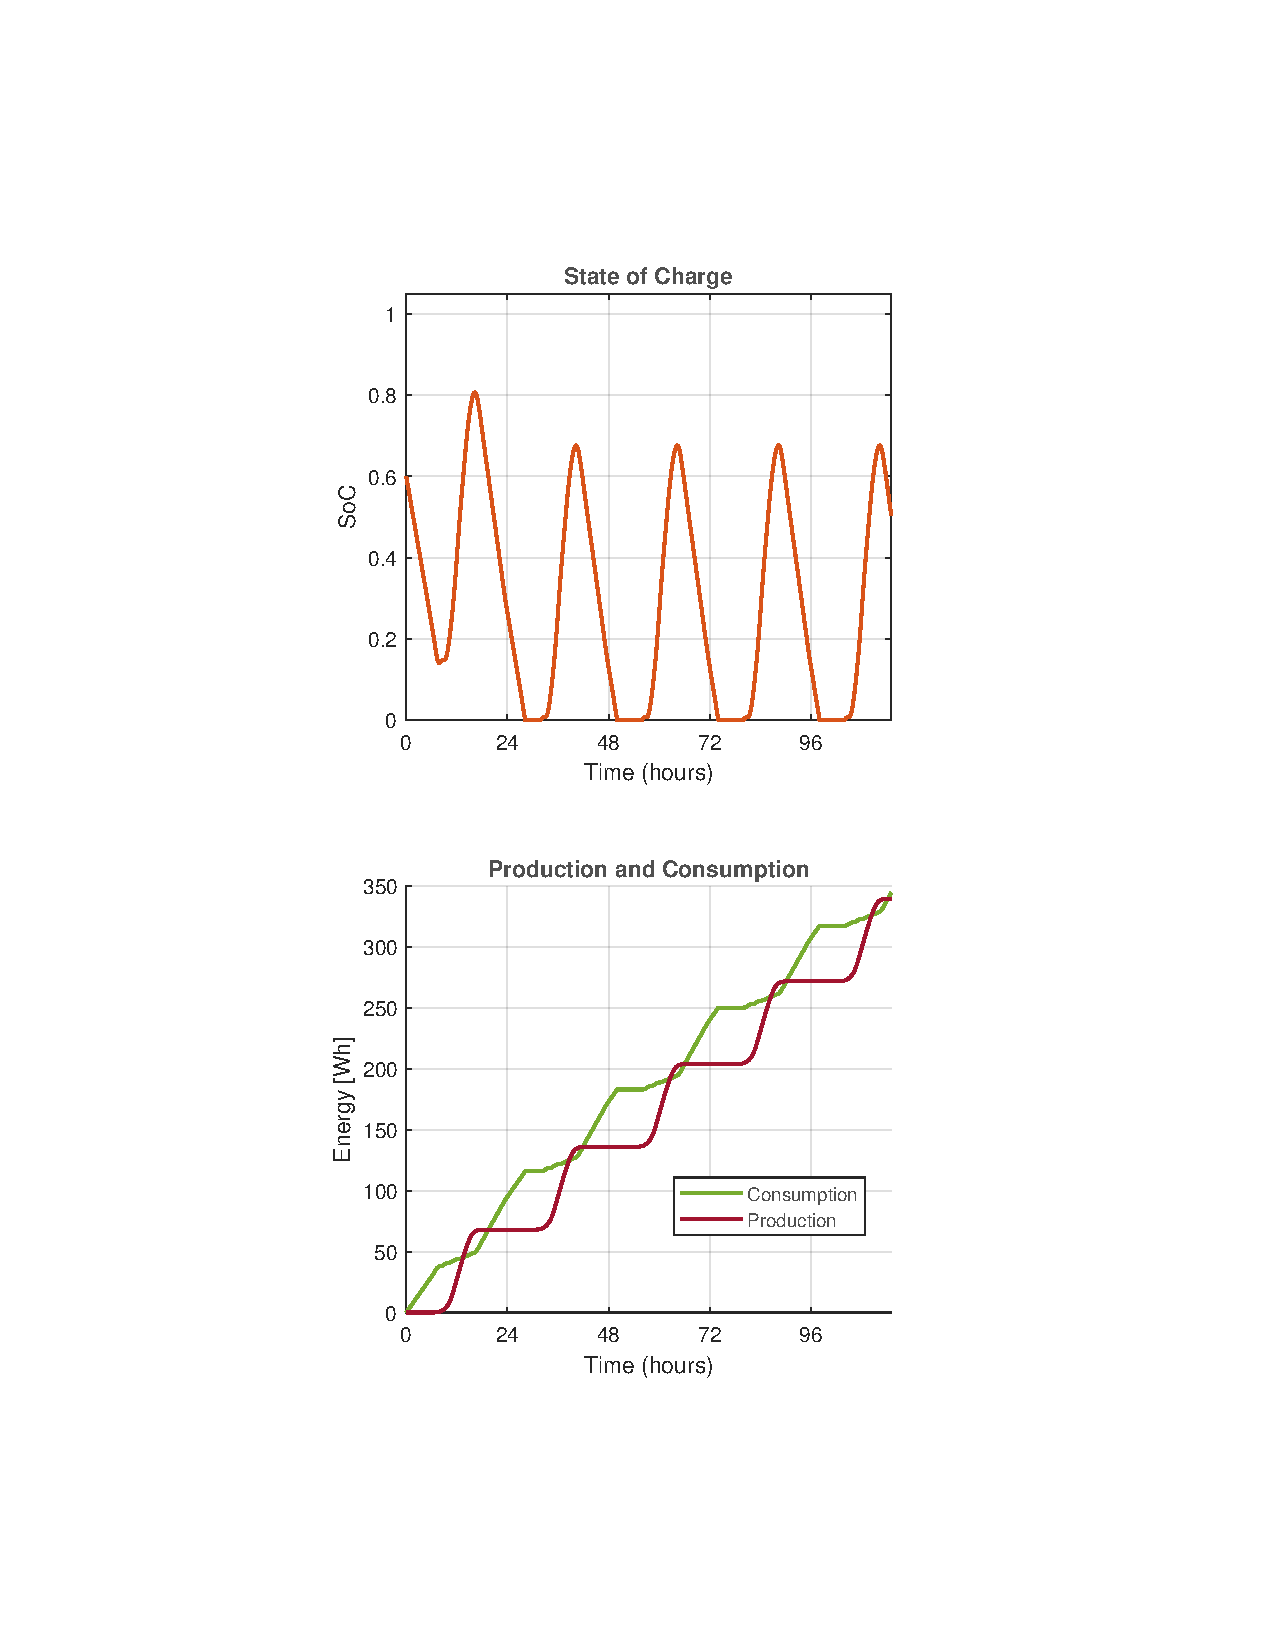
\includegraphics[width=\linewidth]{photos/Winter_SOC&Consumption_with_all_loss_5Days_800System.pdf} %% Gjer denna om til kryss og sirkel
        \captionsetup{font=footnotesize} % Or footnotesize, etc.
        \caption{BH 800 System SoC, production and consumption for winter data. Soiling 10\%, general transmission loss 14\% and effectiveness $\eta$ 79\%.}
        \label{result:fig:800_winter_soc}
    \end{figure}
\end{minipage}

Here we see all three of the systems hit an empty battery in under five days. All systems have full utilization rate based on their consumption. From the question: \textit{Does the battery ever run out, and what does it take to happen?}, the average answer was 2.5 times per year. Using this data, we can assume that the consumption changes according to the production. When cloudy or rainy weather reduces the production, the user reduce their consumption accordingly. 

\newpage
\section{Economical analysis}
On table \ref{tab:energy_summary} we find the annual production and consumption of each of the systems, according to their system specific data from section \ref{sec:systemspesificdata}. Consumption will for some systems match the production, when the system uses all the energy it produces. System BH 300 consumes all of it's production in both winter and summer months, which matches what we see from the simulations. The other systems has some excess production in at least one season. 

\begin{table}[H]
    \centering
    \begin{tabularx}{\linewidth}{|C|S[table-format=5.0]|S[table-format=5.0]|S[table-format=5.0]|S[table-format=5.0]|S[table-format=5.0]|S[table-format=5.0]|}
    \hline
    \textbf{System Name} & \multicolumn{3}{C|}{\textbf{Production (Wh)}} & \multicolumn{3}{C|}{\textbf{Consumption (Wh)}} \\ \cline{2-7}
     & \textbf{Winter} & \textbf{Summer} & \textbf{Annual} & \textbf{Winter} & \textbf{Summer} & \textbf{Annual} \\ \hline
    BH 800 (40Wpp) & 12147 & 21048 & \cellcolor{lightgray}33195 & 8445 & 7759 & \cellcolor{lightgray}16204 \\ \hline
    BH 600 (20Wpp) & 6073 & 10524 & \cellcolor{lightgray}16598 & 6073 & 6466 & \cellcolor{lightgray}12539 \\ \hline
    BH 300 (10Wpp) & 3037 & 5262 & \cellcolor{lightgray}8299 & 3037 & 5262 & \cellcolor{lightgray}8299 \\ \hline
    \end{tabularx}
    \caption{Yearly energy yield for each system based on total production and actual consumption. Sectioned into summer and winter months.}
    \label{tab:energy_summary}
\end{table}
With this data, we can analyze the LCOE and Payback time. Doing an annual calculation for both of these metrics is the most common, and with the data from the table we can do an individual evaluation of all the systems. 

\subsection{LCOE}
In tables \ref{tab:lcoe_qty_prod_5_condensed} and \ref{tab:lcoe_qty_cons_5_condensed} we find the LCOE for the systems with a 5\% discount rate. In tables \ref{tab:lcoe_qty_prod_75_condensed} and \ref{tab:lcoe_qty_cons_75_condensed}, we find for 7.5\%. Lastly the LCOE without discount is shown in table \ref{tab:lcoe_qty_prod_no_discount_condensed}, to compare against similar projects that don't use discount rate. The basis for lifetime is from section \ref{chap:method:sec:LCOE}, but is rounded to whole years. Costs are gathered from table \ref{table:SHS_cost}, where only the quantity price is used. The calculation of LCOE is based on equation \eqref{eq:LCOEfirst}. 

The tables take into account two sets of energy data, both the produced and the consumed. This will compare the potential of the system towards the cost, as well as the actual usage of the system towards the cost. There is also a leap in the lifetime that is shown. Systems are designed for a lifetime of 6-7 years, and at least 2000 cycles. As explained in section \ref{chap:method:sec:LCOE} this is can be under 6 years, which is why 5 years is added. 25 years is 9000 cycles, which was also found in section \ref{chap:method:sec:LCOE} to be the maximum for a battery. 
\small % Apply to the entire set of tables for better fitting

%\noindent % Ensure no paragraph indentation before the minipages
\begin{minipage}[t]{0.45\textwidth}
\centering % Center content within this minipage

% --- Tables for 5% Discount Rate (Left Column) ---

% Table 1: Quantity Price from Production (5% Discount)
\begin{table}[H]
\centering
\begin{tabularx}{\linewidth}{|>{\RaggedRight\hsize=0.25\hsize}X|>{\Centering\hsize=0.25\hsize}X|>{\Centering\hsize=0.25\hsize}X|>{\Centering\hsize=0.25\hsize}X|}
\hline
 \textbf{Lifetime}& \textbf{BH 300} & \textbf{BH 600} & \textbf{BH 800} \\
\hline
\textbf{$L_{5}$} & 28.8 & 18.6 & 12.9 \\ \hline
\textbf{$L_{6}$} & 24.5 & 15.8 & 11.0 \\ \hline
\textbf{$L_{7}$} & 21.5 & 13.9 & 9.6 \\ \hline
\textbf{$L_{8}$} & 19.3 & 12.4 & 8.6 \\ \hline
\textbf{$L_{25}$} & 8.8 & 5.7 & 4.0 \\ \hline
\end{tabularx}
\caption{LCOE for total production with $r=0.05$. Values in EUR/kWh.}
\label{tab:lcoe_qty_prod_5_condensed}
\end{table}

% Table 2: Quantity Price from Consumption (5% Discount)
\begin{table}[H]
\centering
\begin{tabularx}{\linewidth}{|>{\RaggedRight\hsize=0.25\hsize}X|>{\Centering\hsize=0.25\hsize}X|>{\Centering\hsize=0.25\hsize}X|>{\Centering\hsize=0.25\hsize}X|}
\hline
 \textbf{Lifetime}& \textbf{BH 300} & \textbf{BH 600} & \textbf{BH 800} \\
\hline
\textbf{$L_{5}$} & 28.8 & 24.6 & 26.4 \\ \hline
\textbf{$L_{6}$} & 24.5 & 20.9 & 22.5 \\ \hline
\textbf{$L_{7}$} & 21.5 & 18.4 & 19.7 \\ \hline
\textbf{$L_{8}$} & 19.3 & 16.5 & 17.7 \\ \hline
\textbf{$L_{25}$} & 8.8 & 7.5 & 8.1 \\ \hline
\end{tabularx}
\caption{LCOE for actual consumption with $r=0.05$. Values in EUR/kWh.}
\label{tab:lcoe_qty_cons_5_condensed}
\end{table}

\end{minipage}\hfill % Separator between left and right columns
\begin{minipage}[t]{0.45\textwidth}
\centering % Center content within this minipage

% --- Tables for 7.5% Discount Rate (Right Column) ---

% Table 3: Quantity Price from Production (7.5% Discount)
\begin{table}[H]
\centering
\begin{tabularx}{\linewidth}{|>{\RaggedRight\hsize=0.25\hsize}X|>{\Centering\hsize=0.25\hsize}X|>{\Centering\hsize=0.25\hsize}X|>{\Centering\hsize=0.25\hsize}X|}
\hline
 \textbf{Lifetime}& \textbf{BH 300} & \textbf{BH 600} & \textbf{BH 800} \\
\hline
\textbf{$L_{5}$} & 30.8 & 19.9 & 13.8 \\ \hline
\textbf{$L_{6}$} & 26.5 & 17.1 & 11.9 \\ \hline
\textbf{$L_{7}$} & 23.5 & 15.2 & 10.5 \\ \hline
\textbf{$L_{8}$} & 21.3 & 13.7 & 9.5 \\ \hline
\textbf{$L_{25}$} & 11.2 & 7.2 & 5.0 \\ \hline
\end{tabularx}
\caption{LCOE for total production with $r=0.075$. Values in EUR/kWh.}
\label{tab:lcoe_qty_prod_75_condensed}
\end{table}

% Table 4: Quantity Price from Consumption (7.5% Discount)
\begin{table}[H]
\centering
\begin{tabularx}{\linewidth}{|>{\RaggedRight\hsize=0.25\hsize}X|>{\Centering\hsize=0.25\hsize}X|>{\Centering\hsize=0.25\hsize}X|>{\Centering\hsize=0.25\hsize}X|}
\hline
 \textbf{Lifetime}& \textbf{BH 300} & \textbf{BH 600} & \textbf{BH 800} \\
\hline
\textbf{$L_{5}$} & 30.8 & 26.3 & 28.2 \\ \hline
\textbf{$L_{6}$} & 26.5 & 22.7 & 24.3 \\ \hline
\textbf{$L_{7}$} & 23.5 & 20.1 & 21.6 \\ \hline
\textbf{$L_{8}$} & 21.3 & 18.2 & 19.5 \\ \hline
\textbf{$L_{25}$} & 11.2 & 9.5 & 10.2 \\ \hline
\end{tabularx}
\caption{LCOE for actual consumption with $r=0.075$. Values in EUR/kWh.}
\label{tab:lcoe_qty_cons_75_condensed}
\end{table}

\end{minipage}

\vspace{1em} % Add some vertical space before the next table, adjust as needed

% --- Table for No Discount Rate (Centered Below) ---
\begin{table}[H]
\centering
\begin{tabularx}{0.5\textwidth}{|>{\RaggedRight\hsize=0.25\hsize}X|>{\Centering\hsize=0.25\hsize}X|>{\Centering\hsize=0.25\hsize}X|>{\Centering\hsize=0.25\hsize}X|}
\hline
 \textbf{Lifetime}& \textbf{BH 300} & \textbf{BH 600} & \textbf{BH 800} \\
\hline
\textbf{$L_{5}$} & 24.9 & 16.1 & 11.1 \\ \hline
\textbf{$L_{6}$} & 20.8 & 13.4 & 9.3 \\ \hline
\textbf{$L_{7}$} & 17.8 & 11.5 & 8.0 \\ \hline
\textbf{$L_{8}$} & 15.6 & 10.0 & 7.0 \\ \hline
\textbf{$L_{25}$} & 5.0 & 3.2 & 2.2 \\ \hline
\end{tabularx}
\caption{LCOE without discount rate ($r=0$) from production. Values in EUR/kWh.}
\label{tab:lcoe_qty_prod_no_discount_condensed}
\end{table}

With a lifetime 8 or less years, the LCOE for a SHS is unprofitable at best. BH 800 fares best in the comparison for energy production, having a lower LCOE than BH 300 and BH 600. As the price of the system is not linear with the size of the panel, it benefits from a marginal increase in panel size compared to marginal price increase. When looking at the consumption data, the systems don't differ as much. BH 600 has the lowest LCOE, with BH 800 being in the middle and BH 300 being the highest. 

\subsection{Payback time}
To find the payback time we use quantity cost, energy consumption and electricity price. In addition, we add the fair price that the participants feel is justified for the system. Payback time is show in figure \ref{result:fig:paybacktime}.


\begin{minipage}[t]{0.65\textwidth} % Adjust width as needed
    \begin{figure}[H]
        \centering
        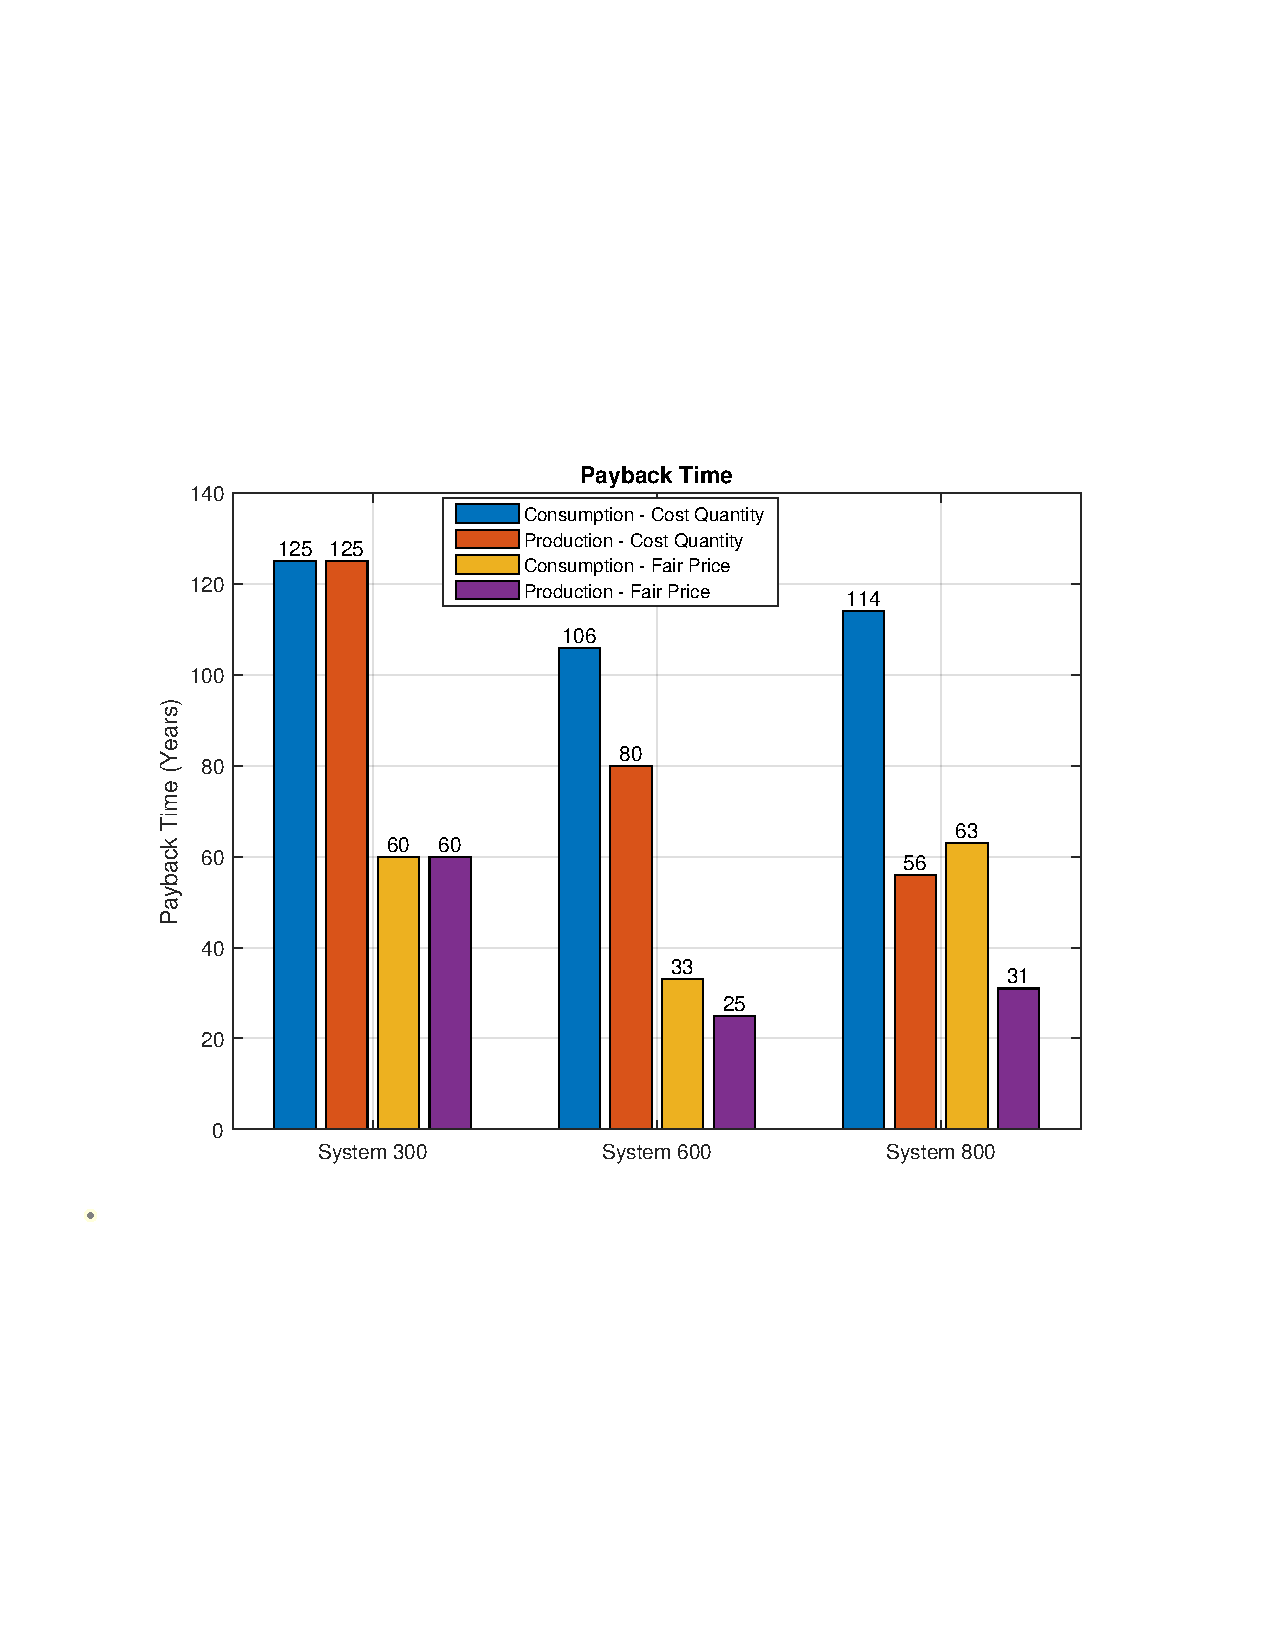
\includegraphics[width=\linewidth]{photos/PaybackTime_comparison_barChart.pdf} %% Gjer denna om til kryss og sirkel
        \captionsetup{font=small}
        \caption{Payback time using actual consumption and total production data from table \ref{tab:energy_summary}, with the electricity price from \ref{method:fig:EU27_elecprice}. Prices are shown in table \ref{tab:fair&quan_price} to the left of the figure.}
        \label{result:fig:paybacktime}
    \end{figure}
\end{minipage}% <--- IMPORTANT: The '%' symbol prevents unwanted horizontal space
%\vspace{0.1\textwidth}
\begin{minipage}[t]{0.35\textwidth}
    \vspace{0.25\textwidth}
    \begin{table}[H]
        \centering
        \small
        \begin{tabularx}{\linewidth}{|>{\RaggedRight\arraybackslash\hsize=0.30\hsize}X|>{\Centering\arraybackslash\hsize=0.30\hsize}X|>{\Centering\arraybackslash\hsize=0.30\hsize}X|}
        \hline
        \multicolumn{3}{|c|}{System prices} \\
        \hline
        System & Quantity price & Fair Price \\
        \hline
        BH 300 & 124 & 60\\ \hline
        BH 600 & 160 & 50  \\ \hline
        BH 800 & 222 & 123 \\ \hline
        \end{tabularx}
        \captionsetup{font=small}
        \caption{Quantity price is gathered from table \ref{table:SHS_cost}. Fair price was a question asked to participants in the interviews, see appendix \ref{apx:ftquestions}. Sample size for fair price is $n<3$, so the data is inaccurate.}
        \label{tab:fair&quan_price} 
    \end{table}
\end{minipage}

Economical payback time ranges from 125 years to 25 years, where 25 years is using the fair price from participants answers. With lifetime of 6-7 years, the economical benefits of the system will not cover the costs during a normal lifetime. Although the system might last longer, the benefits will likely never surpass the cost of the system. This is true regardless of which system we compare. 

\section{Social analysis}

\subsection{Energy sources}
To analyze how SHS has affected households, we wanted to take a look at their current energy sources. Household energy sources can be found on figure \ref{res:soc:householdenergysources}. Although Albania has full grid coverage, we looked at how many of the participants that actually were connected to the grid. Figure \ref{res:soc:gridconnection} shows the results of connection, off-grid and illegal connection.
\begin{figure}[H]
    \centering
    \begin{subfigure}[b]{0.48\textwidth}
        \centering
        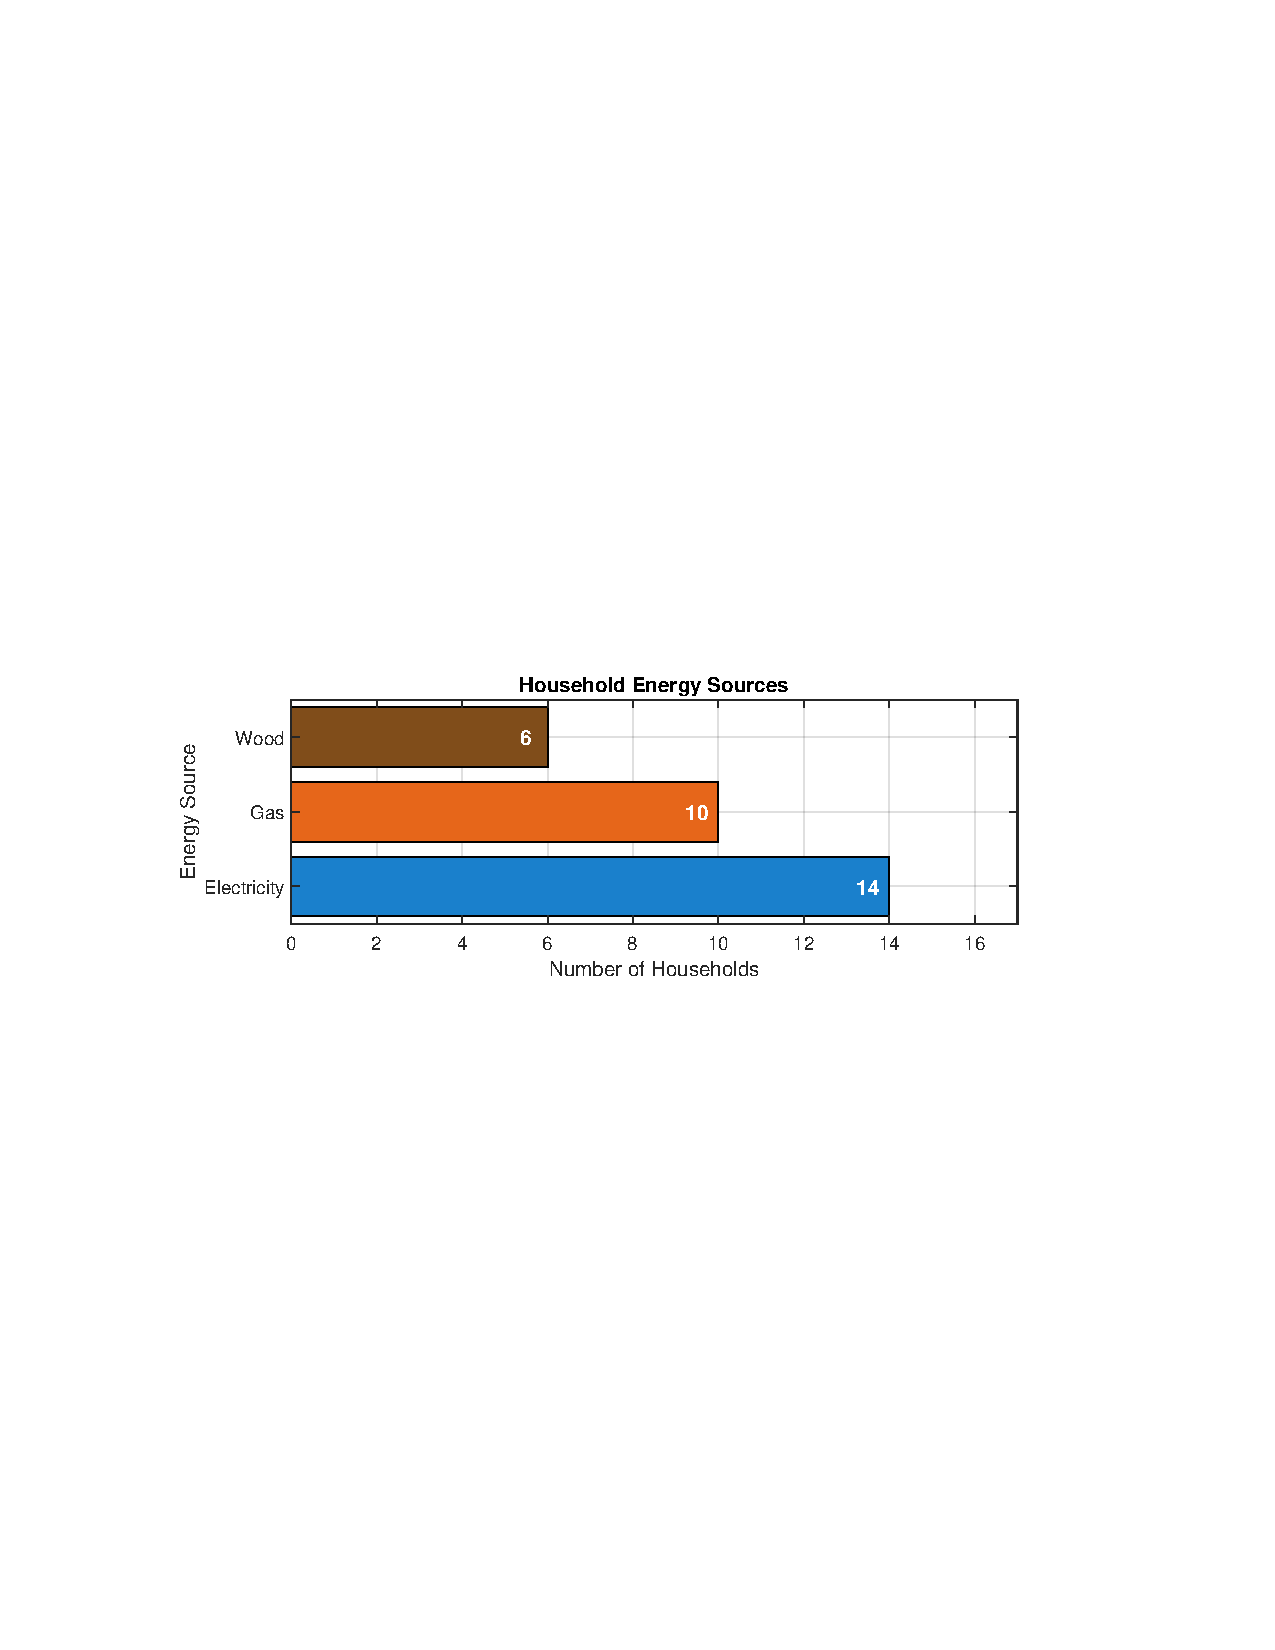
\includegraphics[width=\textwidth]{photos/HouseholdEnergySources.pdf}
        \caption{Numbers are based on 15 interviews of 17 households. Energy sources had various uses, which are not defined here.}
        \label{res:soc:householdenergysources}
    \end{subfigure}
    \hfill
    \begin{subfigure}[b]{0.48\textwidth}
        \centering
        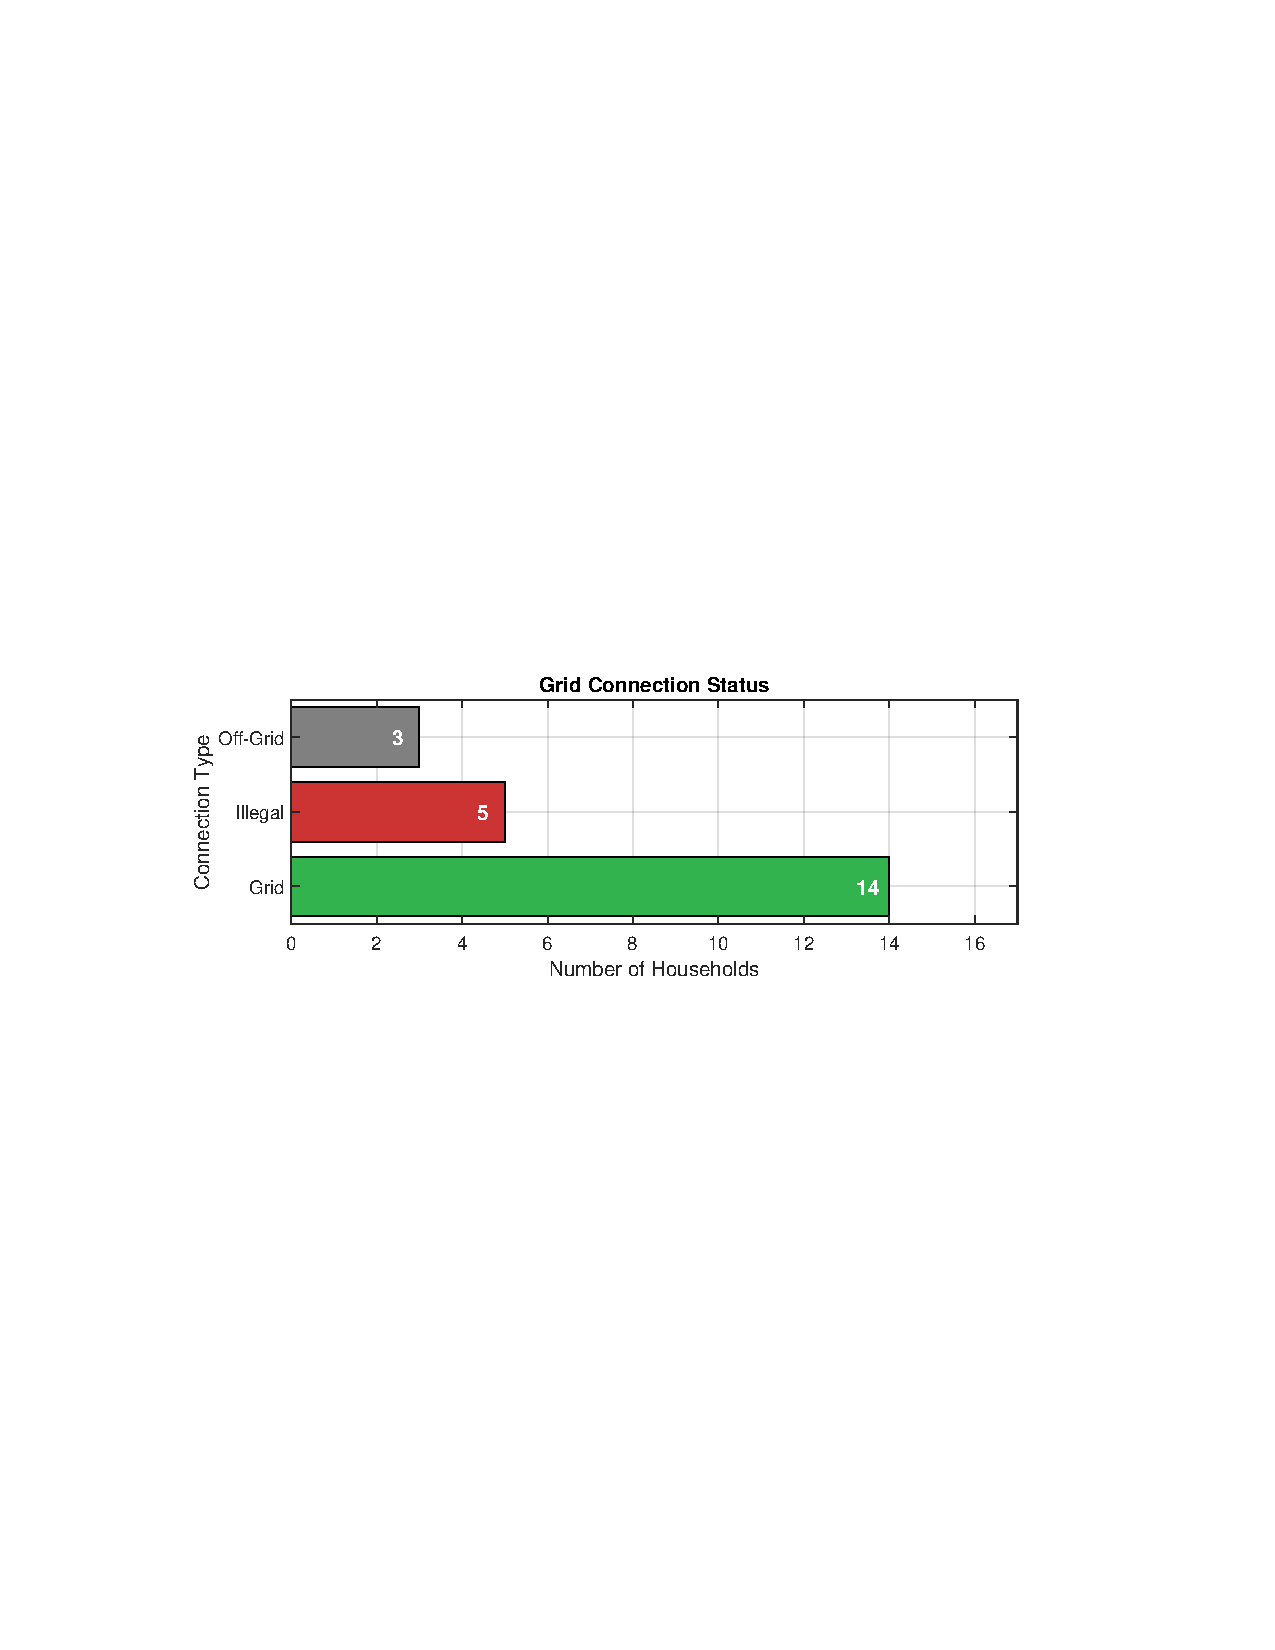
\includegraphics[width=\textwidth]{photos/GridConnection.pdf}
        \caption{Numbers are based on 15 interviews of 17 households. All illegally connected participants where classified as connected to the grid.}
        \label{res:soc:gridconnection}
    \end{subfigure}
\end{figure}
From the graph we see that there were several households that were connected illegally, and some of them were not connected at all. All households that were illegally connected had failed to pay their electricity bill. Either with late payments, or generally incapable of paying for electricity beyond their necessities. Most households had one other energy source than electricity from the grid. Participants viewed the SHS as a separate energy source of electricity. Gas was often used for heating of water and for cooking. Wood was used for general heating or cooking. Most used electricity for washing clothes, TV, sometimes cooking, and sometimes heating water for showers. Among the ones off-grid, two of them were families that had grid connection in the household but were using it for lighting in a shed that had no connection. Two of the illegally connected households had recently connected themselves to the grid illegally, and was previously without electricity. 

\subsection{Power outages and candles}
During the interviews, participants often mentioned regular power outages. Even though we didn't have this as a specific question, we commonly asked this question. The result can be seen in figure \ref{res:soc:poweroutages}. The same thing happened with the SHS replacing candles. Participants often mentioned it as a positive benefit of the systems, and the results can be shown in figure \ref{res:soc:removedcandles}. 

\begin{figure}[H]
    \centering
    \begin{subfigure}[t]{0.48\textwidth}
        \centering
        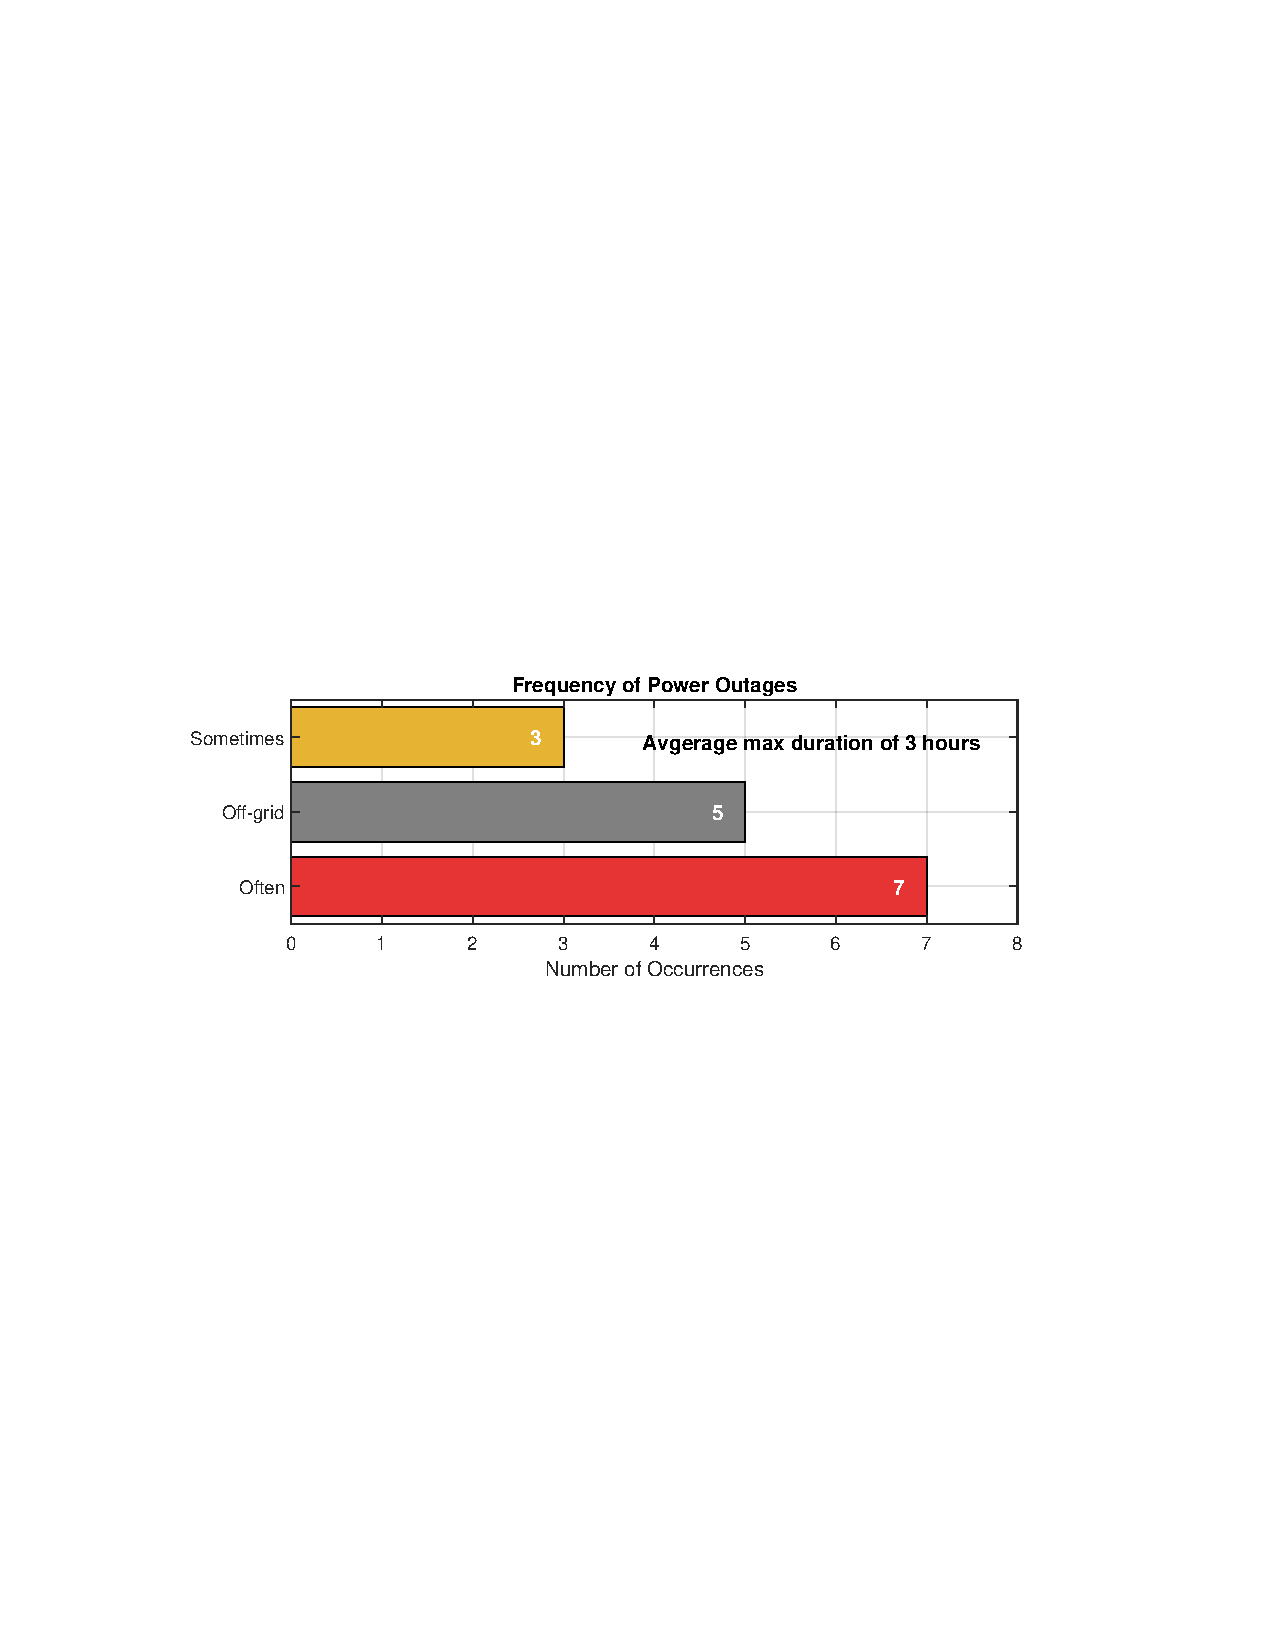
\includegraphics[width=\textwidth]{photos/PowerOutagesFrequency.pdf}
        \caption{"Often" and "Sometimes" are the most accurate data we got from interviews. Some participants referred to often as up to 2-3 times a day. Off-grid are households that had or recently had no grid connection and could not answer for grid stability.}
        \label{res:soc:poweroutages}
    \end{subfigure}
    \hfill
    \begin{subfigure}[t]{0.48\textwidth}
        \centering
        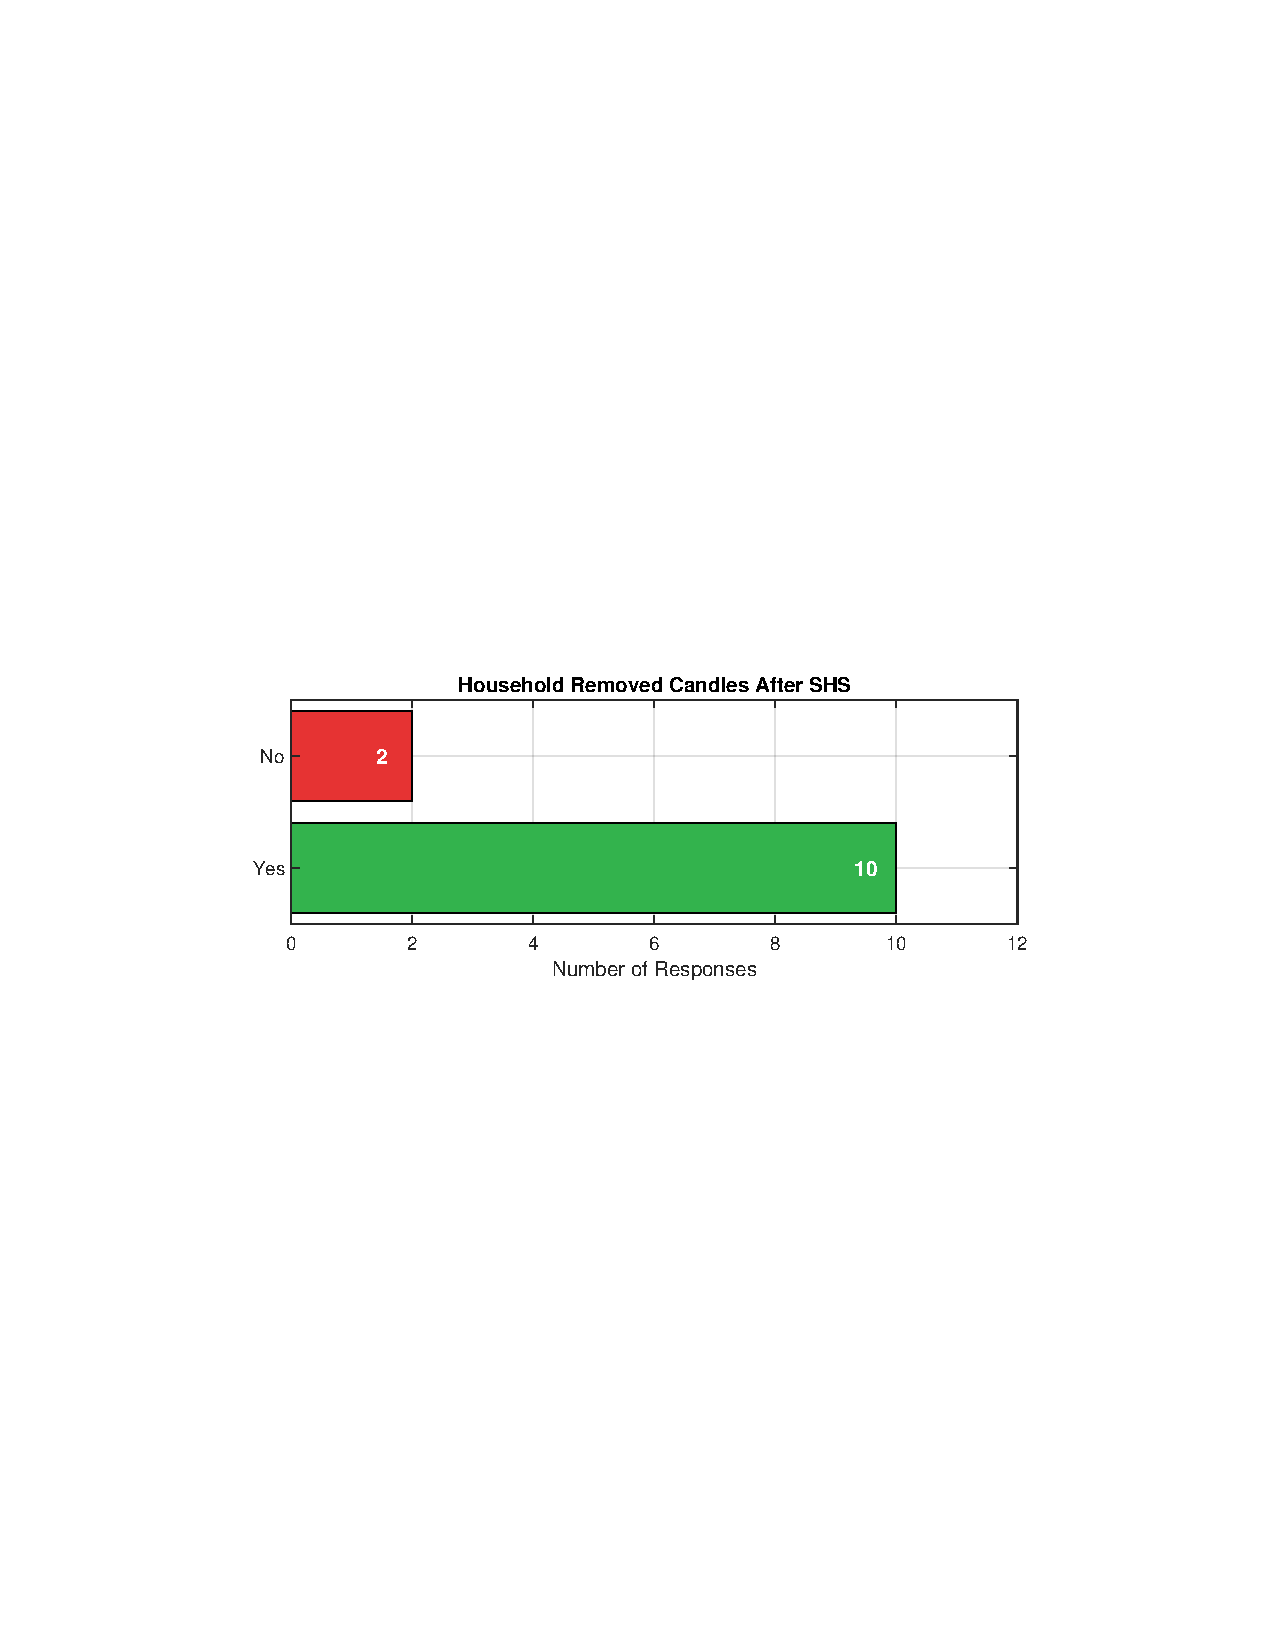
\includegraphics[width=\textwidth]{photos/RemovedCandles.pdf}
        \caption{Based on answers and conversations in interviews. The households that had not gotten candles removed had other systems for emergency lighting, such as battery driven electric lights.}
        \label{res:soc:removedcandles}
    \end{subfigure}
\end{figure}
There seemed to be a high interest for both having an emergency system for power outages, and specifically for being able to removed the need for candles during a power outage. Frequent power outages can create a hard time when having no backup system, and some parts had longer without power than others. Particularly rural areas could have longer power outages than urban areas. One of the main reasons that participants preferred to remove candles, was the fire hazards of having lights inside the house. Participants were acutely aware of the hazards that candles might bring and the consequences of a fire.


\subsection{Household economics}
Participants showed no reluctance to share their incomes and expenditures, giving us the results on figure \ref{res:fig:HouseholdElectricityEconomy}. Some households included more people than others, but this is not shown in the figure. The households are compared regardless of their size, which is why the numbers differ as much. In addition, the numbers for payment reduction are not based on system due to the sample size already being low. 
\begin{figure}[H]
    \centering
    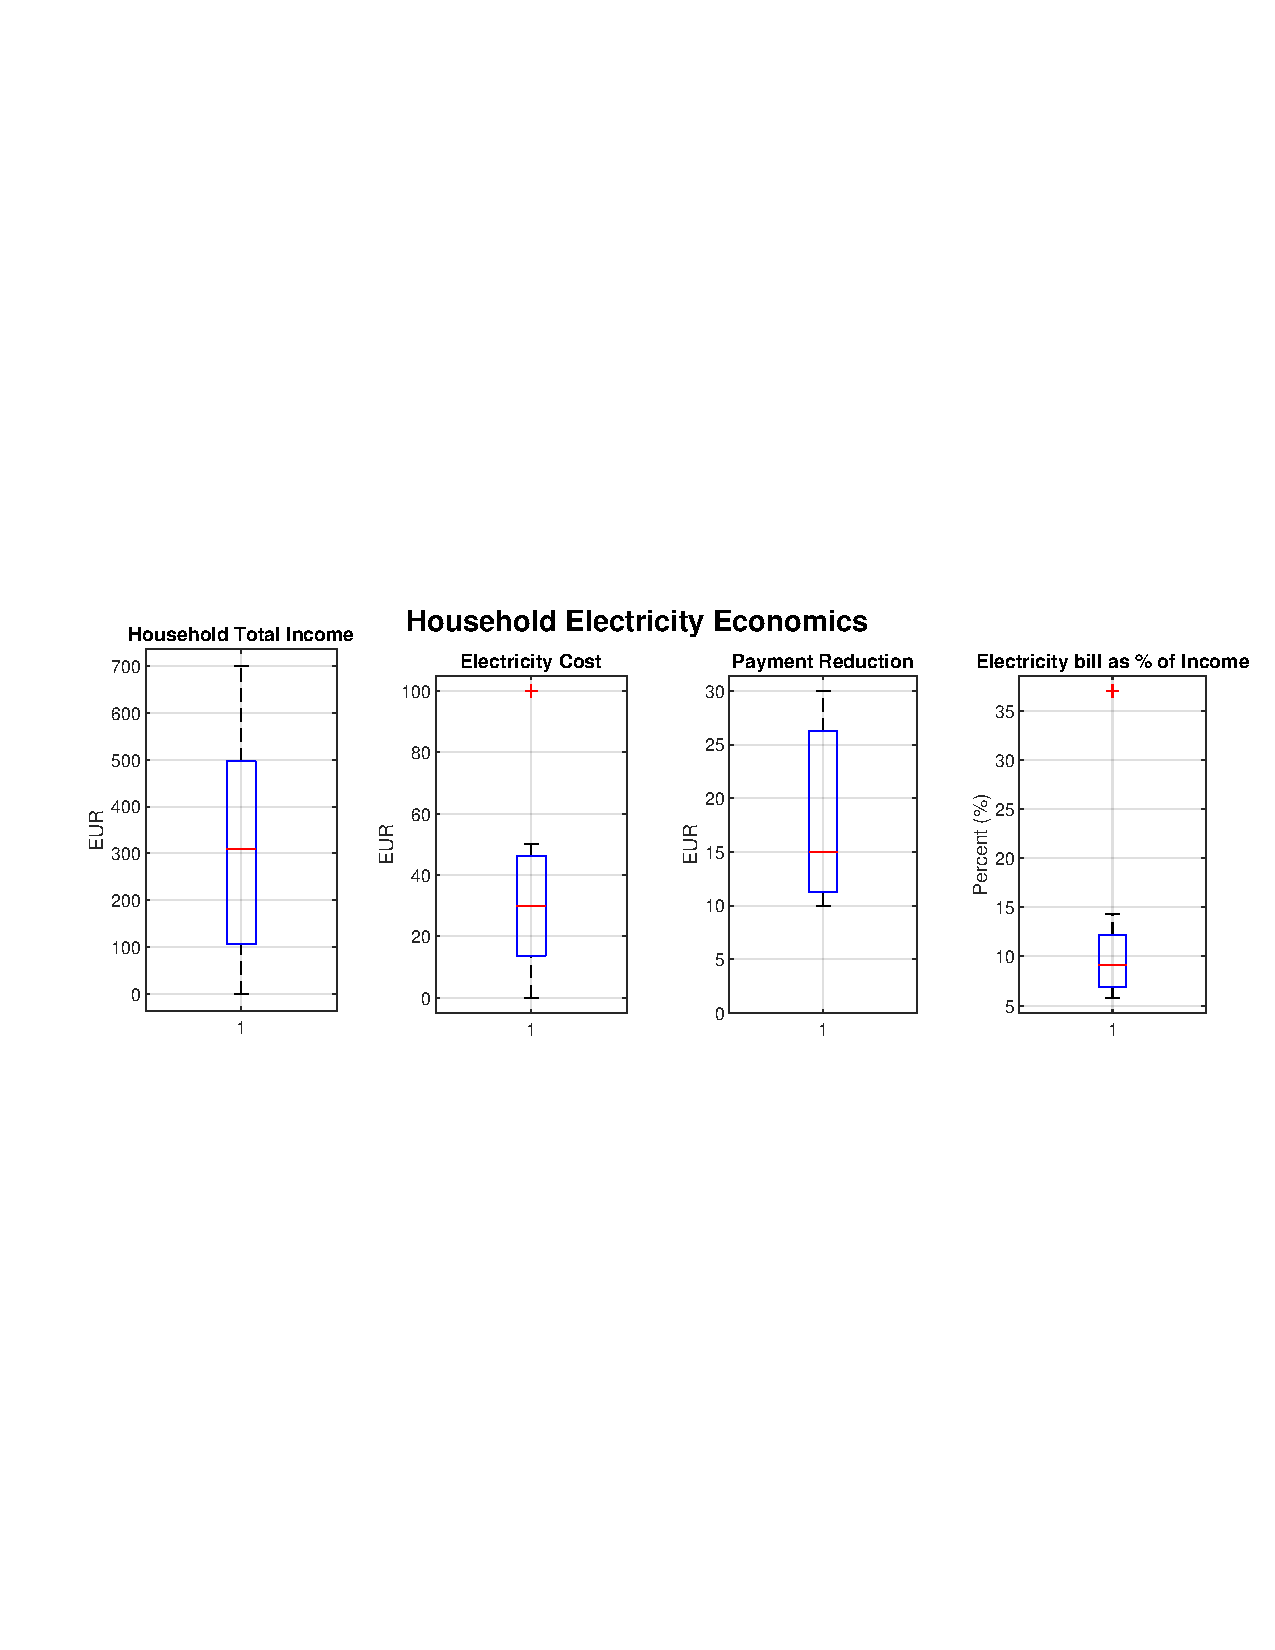
\includegraphics[width=\linewidth]{photos/HouseholdElectricityEconomy.pdf}
    \caption{Box plots of household electricity economy. Numbers are on a monthly basis. Sample sizes are $n=12$, $n=9$, $n=3$ and $n=8$ receptively. Inconsistencies in income and costs sample sizes are due to off-grid and illegal connections, as well as lack of general answers.}
    \label{res:fig:HouseholdElectricityEconomy}
\end{figure}
Total household incomes generally were below 400 EUR a month, which we were told was a normal paycheck for a working person during the field trip. Although not a question asked in the field trip, some people reported how much they had seen a reduction in the electricity bill after installing the SHS. Monthly electricity costs were also taken from a normal month, as the participants often reported being overcharged in the winter months. Some months would charge 5-10 times more than a normal month, based on estimation of consumption and not on actual measurements. This resulted in a complain, which forced the electricity company to measure the correct power consumption and reducing the bill.

Participants showed careful awareness of how much energy they used, taking care not to consume unnecessary energy. The power bill was an average of 8\% of their household income, meaning there was a lot to save on reducing the energy expenditures.

Demographic composition of households in the study differs a lot. Some were elderly people living alone with a pension, and some were families with small children. Figure \ref{res:fig:HouseholdComposition} shows the general composition of a household, and the variation of it. 
\begin{figure}[H]
    \centering
    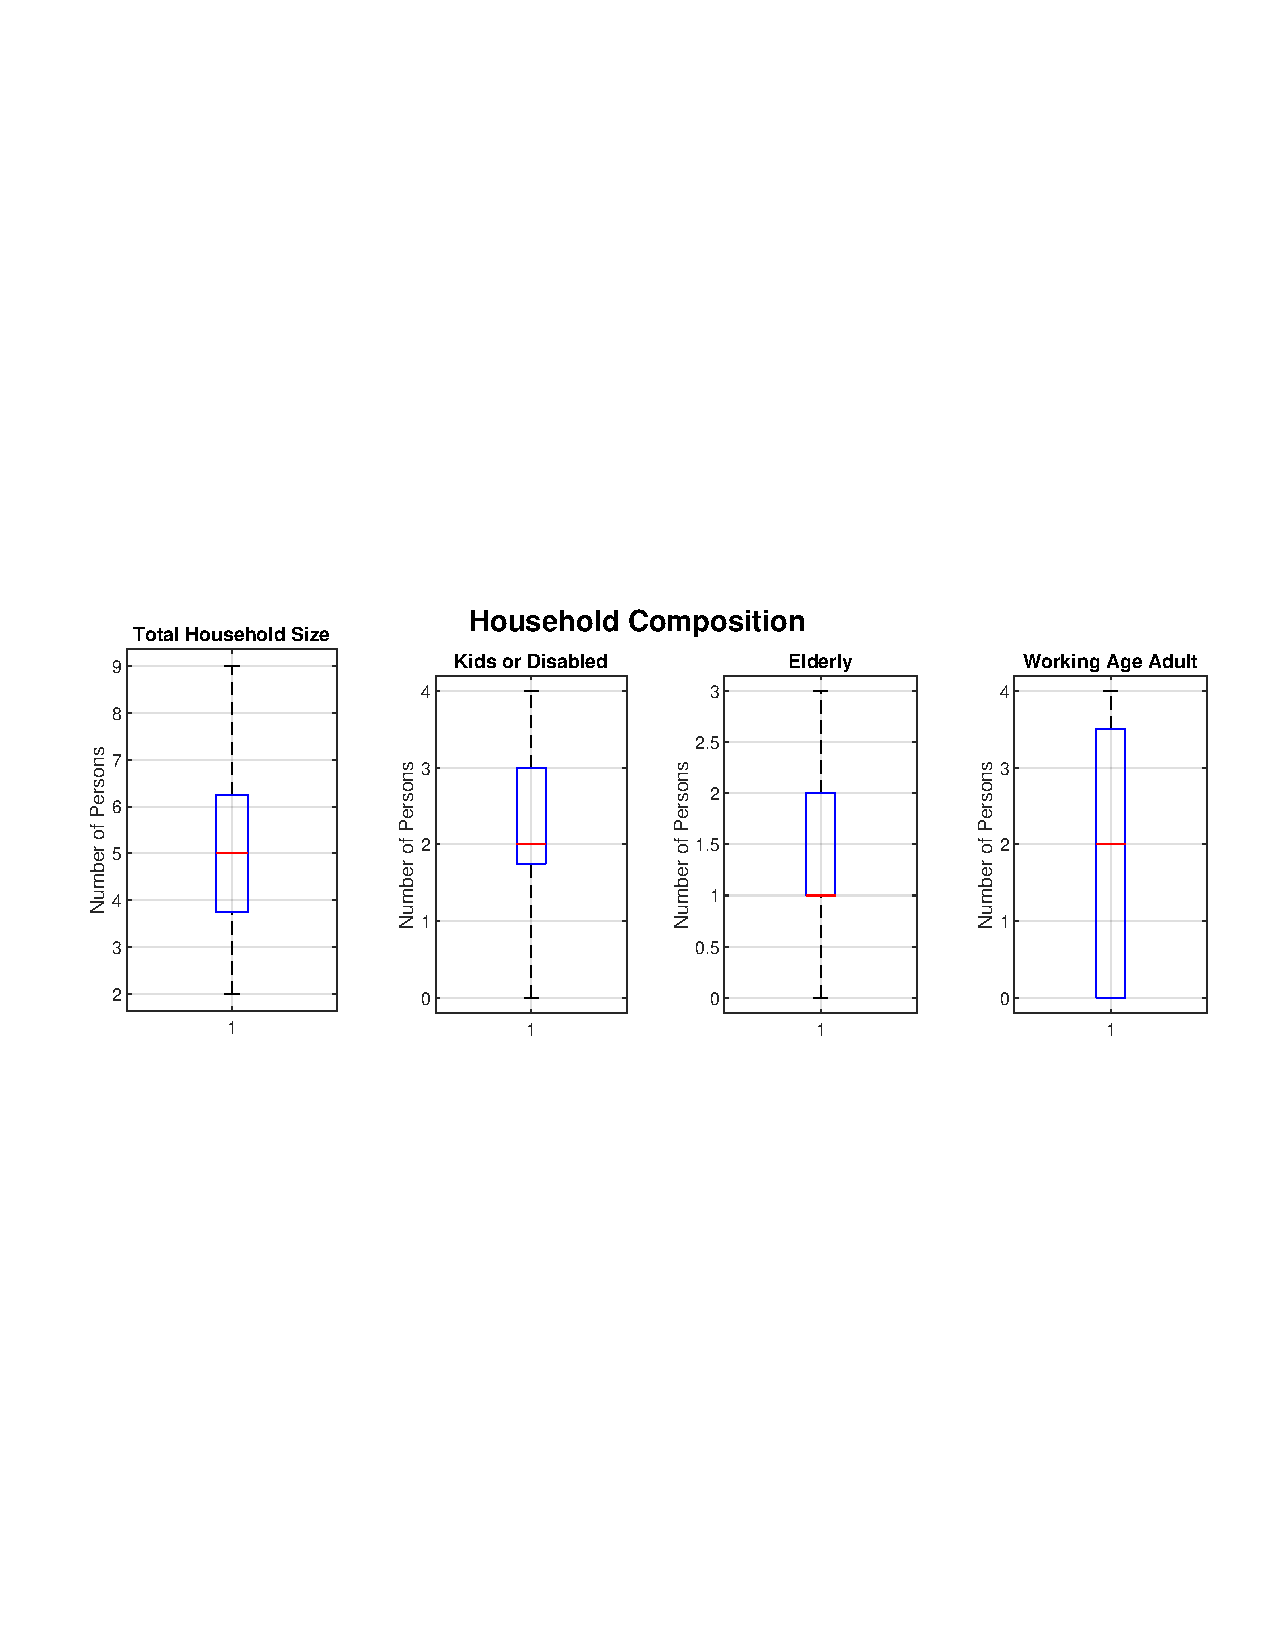
\includegraphics[width=\linewidth]{photos/HouseholdComposition.pdf}
    \caption{Box plots of household composition in terms of kids, elderly and working age adults. Sample sizes are $n=13$ for all plots.}
    \label{res:fig:HouseholdComposition}
\end{figure}
There were several families that included disabled people, as this had been a priority for the project. Households with disabled people reported using the lights throughout the night as a safety in terms of needed care. Small children families often included two adults, where one was working and the other one taking care of the kids. In general there was usually not more than one income per household, besides government support. Most elderly and disabled people received pension from the state as their primary source of income. 

\subsection{Solar power views}
One of the goals of the study was to increase awareness around renewable energy. All of the participants where fond of solar power as an energy source. Most referred to the freedom it had provided them, and how simple it was to use solar power. Contrary to the norm of connecting PV systems to the grid in residential houses, they valued that the system was off-grid. They found the system reliable, and generally understood the concepts of how the solar panel harvested energy for the system. Most people only desired to have more solar power in their household, claiming that they needed a bigger panel. 